%!TEX root = thesis.tex

\section{Manipulation of Demagnetization Integral Operator}
\label{s:Nmanipulation}


\begin{subequations}
\begin{equation}
\textbf{H}(\textbf{r})  = \frac{1}{4\pi}\int\limits_V\nabla\left(\frac{\textbf{r}-\textbf{r}'}{|\textbf{r}-\textbf{r}'|^3}\cdot\textbf{M}(\textbf{r}')\right)\;\mathrm{d}^3r'
\end{equation}
\begin{equation}
\textbf{H}(\textbf{r})  = \frac{1}{4\pi}\int\limits_V\left(\frac{\textbf{r}-\textbf{r}'}{|\textbf{r}-\textbf{r}'|^3}\cdot\textbf{M}(\textbf{r}')\right) \textbf{n}(\textbf{r}')\;\mathrm{d}^3r'
\end{equation}
\begin{equation}
\textbf{H}(\textbf{r})  = \frac{1}{4\pi}\int\limits_V\textbf{n}(\textbf{r}')\left(\frac{\textbf{r}-\textbf{r}'}{|\textbf{r}-\textbf{r}'|^3}\cdot\textbf{M}(\textbf{r}')\right)\;\mathrm{d}^3r'
\end{equation}
\begin{equation}
\textbf{H}(\textbf{r})  = \frac{1}{4\pi}\int\limits_V\textbf{n}(\textbf{r}')\left(\frac{\textbf{r}-\textbf{r}'}{|\textbf{r}-\textbf{r}'|^3}\cdot\textbf{M}(\textbf{r}')\right)\;\mathrm{d}^3r'
\end{equation}
\begin{equation}
\textbf{H}(\textbf{r})  = \frac{1}{4\pi}\int\limits_V\textbf{n}(\textbf{r}')\left(\frac{(\textbf{r}-\textbf{r}')}{|\textbf{r}-\textbf{r}'|^3}^T\textbf{M}(\textbf{r}')\right)\;\mathrm{d}^3r'
\end{equation}
\begin{equation}
\textbf{H}(\textbf{r})  = \frac{1}{4\pi}\int\limits_V\left(\textbf{n}(\textbf{r}')\frac{(\textbf{r}-\textbf{r}')}{|\textbf{r}-\textbf{r}'|^3}^T\right)\textbf{M}(\textbf{r}')\;\mathrm{d}^3r'
\end{equation}
\begin{equation}
\textbf{H}(\textbf{r})  = \frac{1}{4\pi}\int\limits_V\left(\frac{(\textbf{r}-\textbf{r}')}{|\textbf{r}-\textbf{r}'|^3}\textbf{n}(\textbf{r}')^T\right)^T\textbf{M}(\textbf{r}')\;\mathrm{d}^3r'
\end{equation}
\end{subequations}

Here we used the identity $\nabla(\textbf{u}\cdot\textbf{v}) = (\textbf{u}\cdot \nabla)\textbf{v} +  (\textbf{v}\cdot \nabla)\textbf{u} + \textbf{u}\times(\nabla\times\textbf{v}) + \textbf{v}\times(\nabla\times\textbf{u})$ as well as $\int\limits_V \nabla w \,d^3r'=  \oint\limits_{\partial V} w \textbf{n}\,d^2r'$ (for a scalar function $w$) and some simple matrix algebraic manipulations

\section{Proof of Linearity of Integral Equation}
\label{s:LinearityIntegralEquation}

For a specific helix and material we have the following integral equation:

\begin{equation}
\frac{1}{\chi_m}\textbf{M}(\textbf{r})  = -\mathcal{N}(\textbf{M}(\textbf{r})) + \textbf{H}_\text{app}
\end{equation}

We want to prove the linearity of the solution over the applied field. For this sake, we will make the dependance of the solution on the applied field explicit. The solution to this equation is therefore:

\begin{equation}
\textbf{M}(\textbf{r},\textbf{H}_\text{app})
\end{equation}

The next step is to prove linearity of $\textbf{M}(\textbf{r},\textbf{H}_\text{app})$ over $\textbf{H}_\text{app}$. We take first two cases: 


\begin{equation}\label{eq:case1}
\frac{1}{\chi_m}\textbf{M}(\textbf{r},\textbf{H}_\text{app,1})  = -\mathcal{N}(\textbf{M}(\textbf{r},\textbf{H}_\text{app,1})) + \textbf{H}_\text{app,1}
\end{equation}
\begin{equation}\label{eq:case2}
\frac{1}{\chi_m}\textbf{M}(\textbf{r},\textbf{H}_\text{app,2})  = -\mathcal{N}(\textbf{M}(\textbf{r},\textbf{H}_\text{app,2})) + \textbf{H}_\text{app,2}
\end{equation}

with solutions $\textbf{M}(\textbf{r},\textbf{H}_\text{app,1})$ and $\textbf{M}(\textbf{r},\textbf{H}_\text{app,2})$ respectively. By multiplying both equations with a real constant $\alpha$ and $\beta$ respectively and using the linear properties of the integral operator $\mathcal{N(\cdot)}$ it follows that:

\begin{equation}\label{eq:case1alpha}
\frac{1}{\chi_m}\alpha\textbf{M}(\textbf{r},\textbf{H}_\text{app,1})  = -\mathcal{N}(\alpha\textbf{M}(\textbf{r},\textbf{H}_\text{app,1})) + \alpha\textbf{H}_\text{app,1}
\end{equation}
\begin{equation}\label{eq:case2}
\frac{1}{\chi_m}\beta\textbf{M}(\textbf{r},\textbf{H}_\text{app,2})  = -\mathcal{N}(\beta\textbf{M}(\textbf{r},\textbf{H}_\text{app,2})) + \beta\textbf{H}_\text{app,2}
\end{equation}

by adding both equations and again using the algebraic and linearity properties of the integral operator (which has a matrix kernel) it follows that:

\begin{subequations}
\begin{equation}\label{eq:case1alpha}
\frac{1}{\chi_m}(\alpha\textbf{M}(\textbf{r},\textbf{H}_\text{app,1}) + \beta\textbf{M}(\textbf{r},\textbf{H}_\text{app,2}) )   = \end{equation}
\begin{equation}
 -\mathcal{N}(\alpha\textbf{M}(\textbf{r},\textbf{H}_\text{app,1}) + \beta\textbf{M}(\textbf{r},\textbf{H}_\text{app,2})) + (\alpha\textbf{H}_\text{app,1} + \beta\textbf{H}_\text{app,2})
\end{equation}
\end{subequations}

The solution to this is the magnetization field that results of the linear combination of the original fields which can be read clearly from the above equation:

\begin{equation}
\textbf{M}(\textbf{r},\alpha\textbf{H}_\text{app,1} + \beta\textbf{H}_\text{app,2}) = \alpha\textbf{M}(\textbf{r},\textbf{H}_\text{app,1}) + \beta\textbf{M}(\textbf{r},\textbf{H}_\text{app,2})
\end{equation}

Thus, linearity is proven.

\section{Derivation of Demagnetization Matrix for Low Fields}
\label{s:DemagPsi}

We want simplify the following equation:

\begin{equation}
N(\textbf{r}) := -H_d(\textbf{r})\,M(\textbf{r})^{-1}
\end{equation}

with: 

By using the following definitions:

\begin{subequations}
\begin{equation}
M(\textbf{r}) := [\textbf{M}_1(\textbf{r}), \textbf{M}_2(\textbf{r}), \textbf{M}_3(\textbf{r})]
\end{equation}
\begin{equation}
H_\text{app} := [\textbf{H}_{\text{app},1}, \textbf{H}_{\text{app},2}, \textbf{H}_{\text{app},3}]
\end{equation}
\begin{equation}
H_\text{d} := [\textbf{H}_{\text{d},1}, \textbf{H}_{\text{d},2}, \textbf{H}_{\text{d},3}]
\end{equation}
\end{subequations}

where:

\begin{equation}
\textbf{M}_i(\textbf{r}) = \Psi(\textbf{r})\textbf{H}_\text{app,i} \qquad i = 1,2,3
\end{equation}

and from the integral equation follows:


\begin{equation}
\textbf{H}_{d,i}(\textbf{r}) = \mathcal{N}(\textbf{r},\textbf{M}_i(\textbf{r}))\textbf{H}_\text{app,i} \qquad i = 1,2,3
\end{equation}

which simplifies to the following\footnote{Using our integral equation $\frac{1}{\chi_m}\Psi(\textbf{r}) = -\mathcal{N}(\textbf{r},\Psi(\textbf{r}))  + I$}:
\begin{equation}
\textbf{H}_{d,i}(\textbf{r}) = \left(\frac{1}{\chi_m}\Psi(\textbf{r})-I\right)\textbf{H}_\text{app,i} \qquad i = 1,2,3
\end{equation}

our tensor is now:

\begin{subequations}
\begin{equation}
N(\textbf{r}) := -H_d(\textbf{r})\,M(\textbf{r})^{-1} 
\end{equation}
\begin{equation}
 =- \left(\frac{1}{\chi_m}\Psi(\textbf{r})-I\right)H_\text{app} \left( \Psi(\textbf{r})H_\text{app}\right)^{-1}
\end{equation}
\begin{equation}
 = -\left(\frac{1}{\chi_m}\Psi(\textbf{r})-I\right)H_\text{app} H_\text{app}^{-1}\Psi(\textbf{r})^{-1}
\end{equation}
\begin{equation}
 = -\left(\frac{1}{\chi_m}\Psi(\textbf{r})-I\right)\Psi(\textbf{r})^{-1}
\end{equation}
\begin{equation}
 = -\left(\frac{1}{\chi_m}I-\Psi(\textbf{r})^{-1}\right)
\end{equation}
\begin{equation}
 = \Psi(\textbf{r})^{-1}-\frac{1}{\chi_m}I
\end{equation}
\end{subequations}

\clearpage

\section{Simulation Properties of Helices}

\subsection{Full magnetic}
\subsubsection{Geometry}

Description: Here, the geometry was created with the included COMSOL geometry for helices. (See Figure \ref{fig:COMSOLfull})

\begin{figure}[ht]
	\centering
  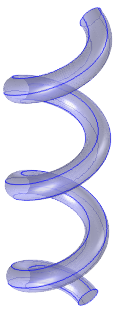
\includegraphics[width=0.15\textwidth]{Pictures/COMSOLfull.png}
	\caption{Example of 3D Geometry in COMSOL of Fully Magnetic Helix}
	\label{fig:COMSOLfull}
\end{figure}


Helix index: $n = 1,2,...,10$\\
Number of Coils: $k = 3$\\
Filament diameter: $d =  3\mu$m\\
Helix height: $h = h_\text{min} + (n -1)\frac{h_\text{max}-h_\text{min}}{9}$\\
Helix diameter: $D = \frac{1}{\pi}\sqrt{\left(\frac{4\cdot v_\text{nom}}{k\cdot \pi \cdot d_\text{nom}^2}\right)^2 - h^2}$\\\\
with:\\\\
$v_\text{nom} = \frac{1}{4}\pi \cdot d_\text{nom}^2 k \sqrt{h_\text{nom}^2+\pi\cdot D_\text{nom}^2} $\\
$d_\text{nom} = 3\mu$m\\
$D_\text{nom} = 10\mu$m\\
$h_\text{min} = 3\mu$m\\
$h_\text{max} = 32.97\mu$m\\
$h_\text{nom} = 10\mu$m

\subsubsection{Meshing Parameters}
COMSOL Predefined: Extremely fine

\subsection{Thin shell}
\subsubsection{Geometry}

Description: Here, the geometry was created with the included COMSOL geometry for helices. First a helix as created with the parametes below and afterwards an identical one with a filament diameter of $d = 3\mu\text{m} - 300$nm was substracted from it (See Figure \ref{fig:COMSOLthin}).

\begin{figure}[ht]
	\centering
  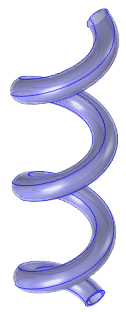
\includegraphics[width=0.15\textwidth]{Pictures/COMSOLthin.png}
	\caption{Example of 3D Geometry in COMSOL of Thin Coated Magnetic Helix}
	\label{fig:COMSOLthin}
\end{figure}

Helix index: $n = 1,2,...,10$\\
Number of Coils: $k = 3$\\
Filament diameter: $d =  3\mu$m\\
Helix height: $h = h_\text{min} + (n -1)\frac{h_\text{max}-h_\text{min}}{9}$\\
Helix diameter: $D = \frac{1}{\pi}\sqrt{\left(\frac{4\cdot v_\text{nom}}{k\cdot \pi \cdot d_\text{nom}^2}\right)^2 - h^2}$\\
Shell thickness: $s = 300$nm\\\\
with:\\\\
$v_\text{nom} = \frac{1}{4}\pi \cdot d_\text{nom}^2 k \sqrt{h_\text{nom}^2+\pi\cdot D_\text{nom}^2} $\\
$d_\text{nom} = 3\mu$m\\
$D_\text{nom} = 10\mu$m\\
$h_\text{min} = 3\mu$m\\
$h_\text{max} = 32.97\mu$m\\
$h_\text{nom} = 10\mu$m

\subsubsection{Meshing Parameters}
COMSOL Predefined: Extremely Fine

\subsection{Half Coated shell}
\subsubsection{Geometry}

Description: Here, the geometry was created with the included COMSOL geometry for helices. First a helix with its main axis pointing in z-direction was created with the parametes below and afterwards an identical one with shifted in negative x-direction by $s = 300$nm (See Figure \ref{fig:COMSOLhalf})

\begin{figure}[ht]
	\centering
  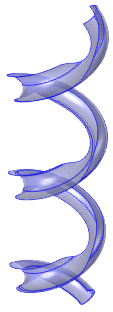
\includegraphics[width=0.15\textwidth]{Pictures/COMSOLhalf.png}
	\caption{Example of 3D Geometry in COMSOL of Half Coated Magnetic Helix}
	\label{fig:COMSOLhalf}
\end{figure}

Helix index: $n = 1,2,...,10$\\
Number of Coils: $k = 3$\\
Filament diameter: $d =  3\mu$m\\
Helix height: $h = h_\text{min} + (n -1)\frac{h_\text{max}-h_\text{min}}{9}$\\
Helix diameter: $D = \frac{1}{\pi}\sqrt{\left(\frac{4\cdot v_\text{nom}}{k\cdot \pi \cdot d_\text{nom}^2}\right)^2 - h^2}$\\
Shift factor: $s = 300$nm\\\\
with:\\\\
$v_\text{nom} = \frac{1}{4}\pi \cdot d_\text{nom}^2 k \sqrt{h_\text{nom}^2+\pi\cdot D_\text{nom}^2} $\\
$d_\text{nom} = 3\mu$m\\
$D_\text{nom} = 10\mu$m\\
$h_\text{min} = 3\mu$m\\
$h_\text{max} = 32.97\mu$m\\
$h_\text{nom} = 10\mu$m

\subsubsection{Meshing parameters}
\begin{tabular}{ | l | l | l | l | l | l | }
\hline
	h & Maximum & Minimum & Maximum   & Curvature  & Resolution \\ 
	 &  element &  element &  element   &  factor & of narrow  \\
	 &   size: &   size: &  growth rate: &   &  regions: \\ \hline
	1.5 & 1.37 & 1.71 & 1.45 & 0.5 & 0.6 \\ \hline
	1.65 & 1.44 & 1.81 & 1.45 & 0.5 & 0.6 \\ \hline
	1.75 & 1.56 & 1.95 & 1.45 & 0.5 & 0.6 \\ \hline
	1.9 & 1.69 & 2.12 & 1.45 & 0.5 & 0.6 \\ \hline
	2 & 1.77 & 2.21 & 1.45 & 0.5 & 0.6 \\ \hline
	2.2 & 1.93 & 2.41 & 1.45 & 0.5 & 0.6 \\ \hline
	2.3 & 2.33 & 2.91 & 1.45 & 0.5 & 0.6 \\ \hline
	2.35 & 2.33 & 2.91 & 1.45 & 0.5 & 0.6 \\ \hline
	2.45 & 2.33 & 2.91 & 1.45 & 0.5 & 0.6 \\ \hline
	2.55 & 2.33 & 2.91 & 1.45 & 0.5 & 0.6 \\ \hline
	2.6 & 2.33 & 2.91 & 1.45 & 0.5 & 0.6 \\ \hline
	2.7 & 2.33 & 2.91 & 1.45 & 0.5 & 0.6 \\ \hline
	2.8 & 2.33 & 2.91 & 1.45 & 0.5 & 0.6 \\ \hline
	3 & 2.33 & 2.91 & 1.45 & 0.5 & 0.6 \\ \hline
	3.2 & 2.33 & 2.91 & 1.45 & 0.5 & 0.6 \\ \hline
	3.3 & 2.33 & 2.91 & 1.45 & 0.5 & 0.6 \\ \hline
	4 & 3.36 & 4.19 & 1.45 & 0.5 & 0.6 \\ \hline
	5 & 4.14 & 5.18 & 1.45 & 0.5 & 0.6 \\ \hline
	6 & 3.4 & 2.47 & 1.45 & 0.5 & 0.6 \\ \hline
	7.2 & 5.87 & 7.34 & 1.45 & 0.5 & 0.6 \\ \hline
	8 & 6.49 & 8.11 & 1.45 & 0.5 & 0.6 \\ \hline
	9.1 & 7.4 & 9.25 & 1.45 & 0.5 & 0.6 \\ \hline
	10 & 7.95 & 9.94 & 1.45 & 0.5 & 0.6 \\ \hline
\end{tabular}

\clearpage

\section{Assumption Assessment of Averaged Demagnetization Field for Low Applied Fields}
\label{s:NMComparison}

We want to analyse in depth the two averaging cases of the demagnetization field for low applied fields by using the matrix formulation:

\begin{equation}
N(\textbf{r}) = \Psi(\textbf{r})^{-1} - \frac{1}{\chi_m}I
\end{equation}

and 

\begin{equation}
\textbf{M}(\textbf{r}) = \Psi(\textbf{r})\textbf{H}_\text{app}
\end{equation}

and we insert it in both cases:

\begin{subequations}
\begin{equation}
\textbf{H}_{d,1} = -\langle N(\textbf{r})\rangle \langle \textbf{M}(\textbf{r})\rangle
\end{equation}
\begin{equation}
 = -\langle \Psi(\textbf{r})^{-1} - \frac{1}{\chi_m}I\rangle \langle \Psi(\textbf{r})\textbf{H}_\text{app} \rangle
\end{equation}
\begin{equation}
 = -\left(\langle \Psi(\textbf{r})^{-1}\rangle - \frac{1}{\chi_m}I\right) \langle \Psi(\textbf{r}) \rangle\textbf{H}_\text{app}
\end{equation}
\begin{equation}
 = -\left(\langle \Psi(\textbf{r})^{-1}\rangle  \langle \Psi(\textbf{r}) \rangle- \frac{1}{\chi_m} \langle \Psi(\textbf{r}) \rangle\right)\textbf{H}_\text{app}
\end{equation}
\end{subequations}
and
\begin{subequations}
\begin{equation}
\textbf{H}_{d,2} = - \langle N(\textbf{r})  \textbf{M}(\textbf{r})\rangle
\end{equation}
\begin{equation}
= - \langle\left( \Psi(\textbf{r})^{-1} - \frac{1}{\chi_m}I \right) \Psi(\textbf{r})\textbf{H}_\text{app}\rangle
\end{equation}
\begin{equation}
= - \langle\left( I - \frac{1}{\chi_m} \Psi(\textbf{r}) \right)\textbf{H}_\text{app}\rangle
\end{equation}
\begin{equation}
= -\left( I - \frac{1}{\chi_m}  \langle\Psi(\textbf{r})\rangle \right)\textbf{H}_\text{app}
\end{equation}
\end{subequations}

The following holds then
\begin{equation}
\textbf{H}_{d,1} \approx \textbf{H}_{d,2}  \Rightarrow \langle \Psi(\textbf{r})^{-1}\rangle  \langle \Psi(\textbf{r}) \rangle \approx I
\end{equation}

In order to assess how good the assumption is, one should further analyse the characteristics of the matrix function $\Psi(\textbf{r})$. Specifically the solutions of the matrix integral equation which describes it. This will be left for further research.

\clearpage

\section{Proof that $N$ and $\chi_a$ share eigenvalues}
\label{s:SameEigen}

We recall the relation between $N$ and $\chi_a$:

\begin{equation}
\chi_a = \left(\frac{1}{\chi_m}I+N\right)^{-1}
\end{equation}

Lets assume that $Q$ is the matrix that diagonalizes $N$ such that $N_\text{diag} = QNQ^{-1}$.

For try to diagonalize now the apparent susceptibility out with the same matrix $Q$:
\begin{subequations}
\begin{equation}
Q \chi_aQ^{-1} 
\end{equation}
\begin{equation}
=Q \left(\frac{1}{\chi_m}I+ N\right)^{-1}Q^{-1} 
\end{equation}
\begin{equation}
= Q\left[Q\left(\frac{1}{\chi_m}I+ N\right)\right]^{-1} 
\end{equation}
\begin{equation}
= Q\left(Q\frac{1}{\chi_m}I+ QN\right)^{-1} 
\end{equation}
\begin{equation}
= \left[\left(Q\frac{1}{\chi_m}I+ QN\right)Q^{-1}\right]^{-1} 
\end{equation}
\begin{equation}
= \left(Q\frac{1}{\chi_m}IQ^{-1}+ QNQ^{-1}\right)^{-1} 
\end{equation}
\begin{equation}
= \left(\frac{1}{\chi_m}QQ^{-1}+ QNQ^{-1}\right)^{-1} 
 \end{equation}
 \begin{equation}
 = \left(\frac{1}{\chi_m}I+ QNQ^{-1}\right)^{-1} 
 \end{equation}
 \begin{equation}
 = \left(\frac{1}{\chi_m}I+ N_\text{diag}\right)^{-1} 
 \end{equation}
\end{subequations} 
 
which is also a diagonal matrix. This means that $Q$ also diagonalizes $\chi_a$ and both matrices share eigenvalues.

\clearpage

\section{Experimental Assessment for Polycristalline Nickel Helices}
\label{s:ExperimentalResults}

\begin{figure}[h]
	\centering
  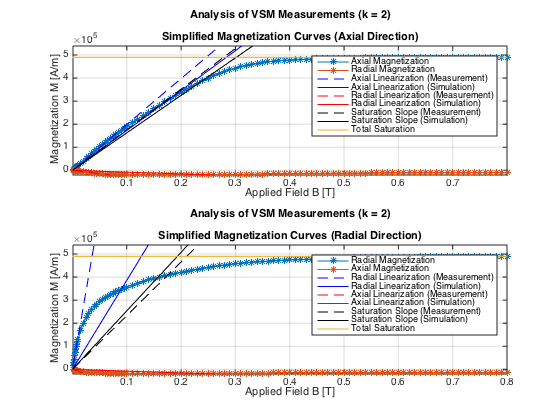
\includegraphics[width=1\textwidth]{Pictures/ExperimentalAssessk2.png}
	\caption{Comparison of simulation and experimental magnetization results for polycristalline nickel macrohelix (k = 2)}
	\label{fig:ExperimentalAssessk2}
\end{figure}

\begin{figure}[h]
	\centering
  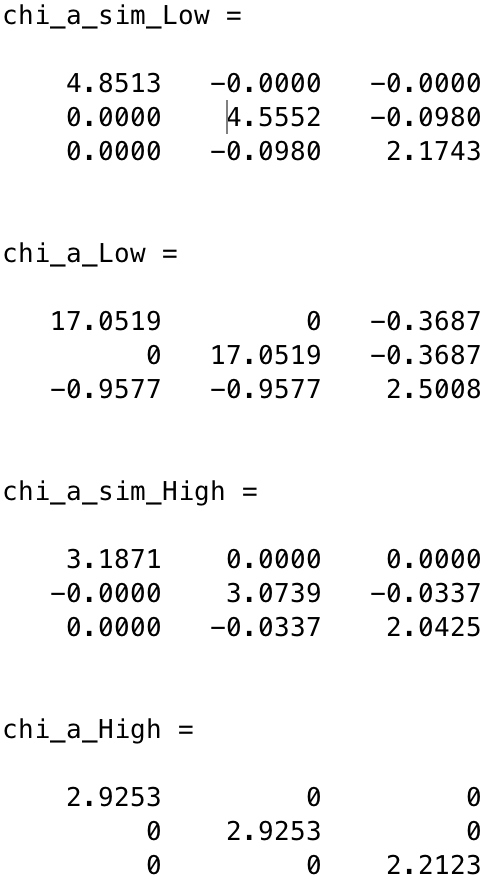
\includegraphics[width=0.25\textwidth]{Pictures/ExperimentalAssessk2chi.png}
	\caption{Comparison of simulation and experimental apparent susceptibilities for high and low fields for polycristalline nickel macrohelix (k = 2)}
	\label{fig:ExperimentalAssessk2chi}
\end{figure}

\begin{figure}[h]
	\centering
  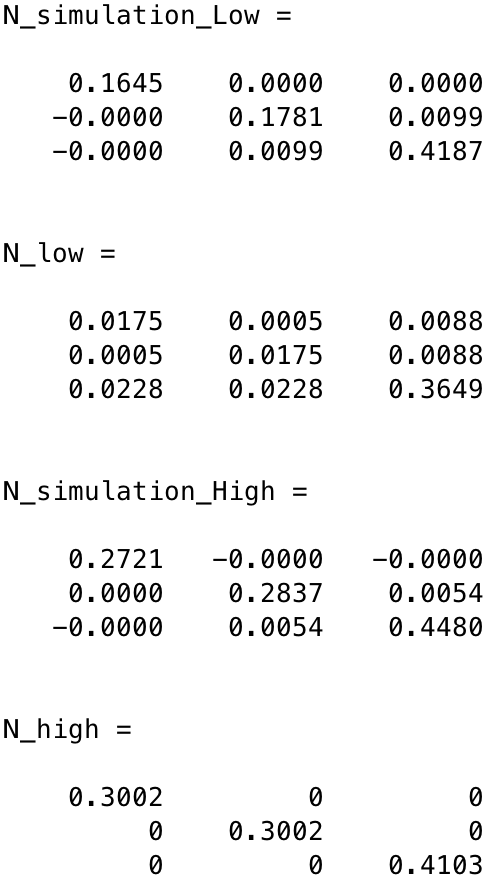
\includegraphics[width=0.25\textwidth]{Pictures/ExperimentalAssessk2N.png}
	\caption{Comparison of simulation and experimental demagnetization matrices for high and low fields for polycristalline nickel macrohelix (k = 2)}
	\label{fig:ExperimentalAssessk2N}
\end{figure}


\begin{figure}[h]
	\centering
  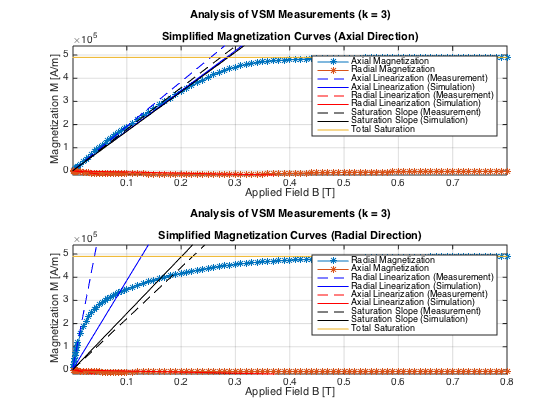
\includegraphics[width=1\textwidth]{Pictures/ExperimentalAssessk3.png}
	\caption{Comparison of simulation and experimental magnetization results for polycristalline nickel macrohelix (k = 3)}
	\label{fig:ExperimentalAssessk3}
\end{figure}

\begin{figure}[h]
	\centering
  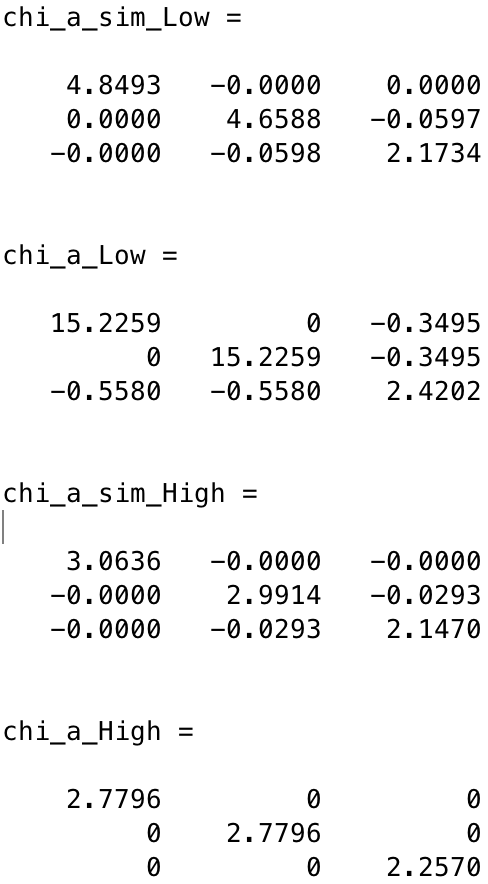
\includegraphics[width=0.25\textwidth]{Pictures/ExperimentalAssessk3chi.png}
	\caption{Comparison of simulation and experimental apparent susceptibilities for high and low fields for polycristalline nickel macrohelix (k = 3)}
	\label{fig:ExperimentalAssessk3chi}
\end{figure}

\begin{figure}[h]
	\centering
  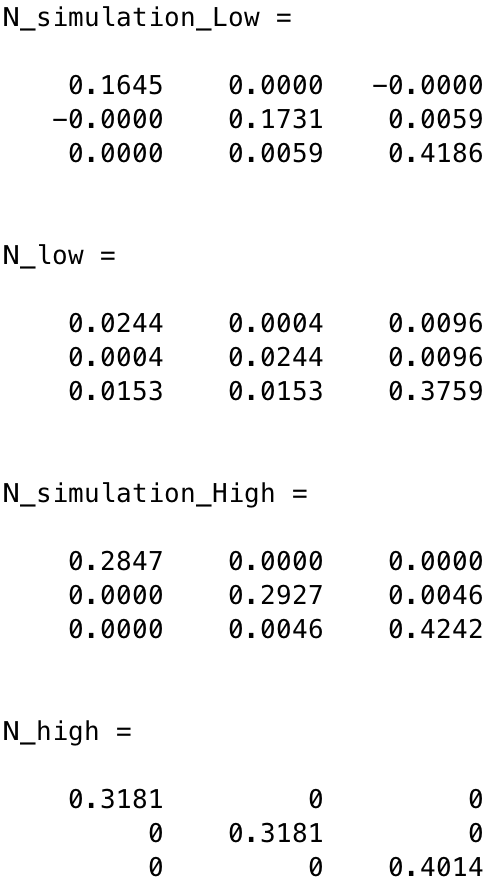
\includegraphics[width=0.25\textwidth]{Pictures/ExperimentalAssessk3N.png}
	\caption{Comparison of simulation and experimental demagnetization matrices for high and low fields for polycristalline nickel macrohelix (k = 3)}
	\label{fig:ExperimentalAssessk3N}
\end{figure}


\begin{figure}[h]
	\centering
  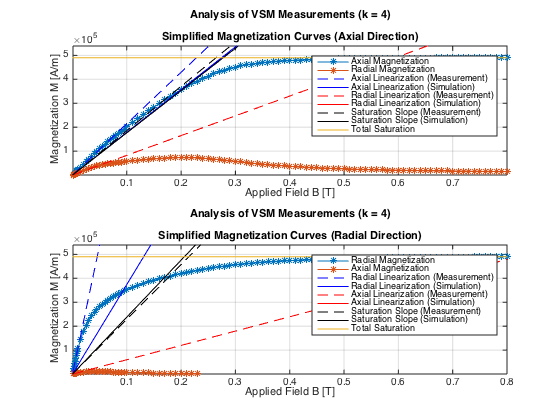
\includegraphics[width=1\textwidth]{Pictures/ExperimentalAssessk4.png}
	\caption{Comparison of simulation and experimental magnetization results for polycristalline nickel macrohelix (k = 4)}
	\label{fig:ExperimentalAssessk4}
\end{figure}

\begin{figure}[h]
	\centering
  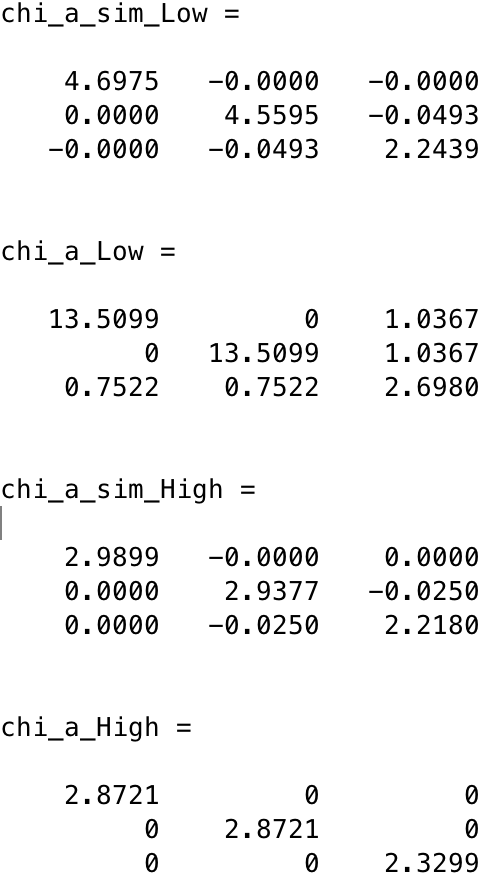
\includegraphics[width=0.25\textwidth]{Pictures/ExperimentalAssessk4chi.png}
	\caption{Comparison of simulation and experimental apparent susceptibilities for high and low fields for polycristalline nickel macrohelix (k = 4)}
	\label{fig:ExperimentalAssessk4chi}
\end{figure}

\begin{figure}[h]
	\centering
  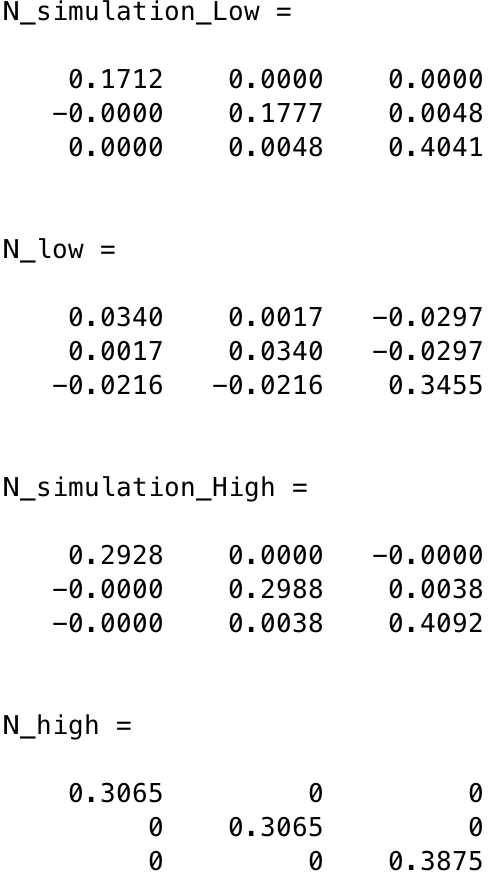
\includegraphics[width=0.25\textwidth]{Pictures/ExperimentalAssessk4N.png}
	\caption{Comparison of simulation and experimental demagnetization matrices for high and low fields for polycristalline nickel macrohelix (k = 4)}
	\label{fig:ExperimentalAssessk4N}
\end{figure}

\begin{figure}[h]
	\centering
  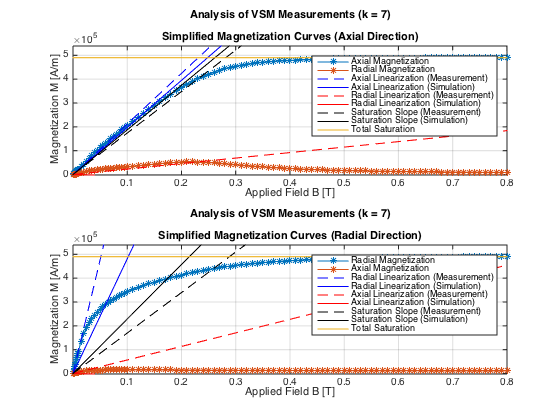
\includegraphics[width=1\textwidth]{Pictures/ExperimentalAssessk7.png}
	\caption{Comparison of simulation and experimental magnetization results for polycristalline nickel macrohelix (k = 7)}
	\label{fig:ExperimentalAssessk7}
\end{figure}

\begin{figure}[h]
	\centering
  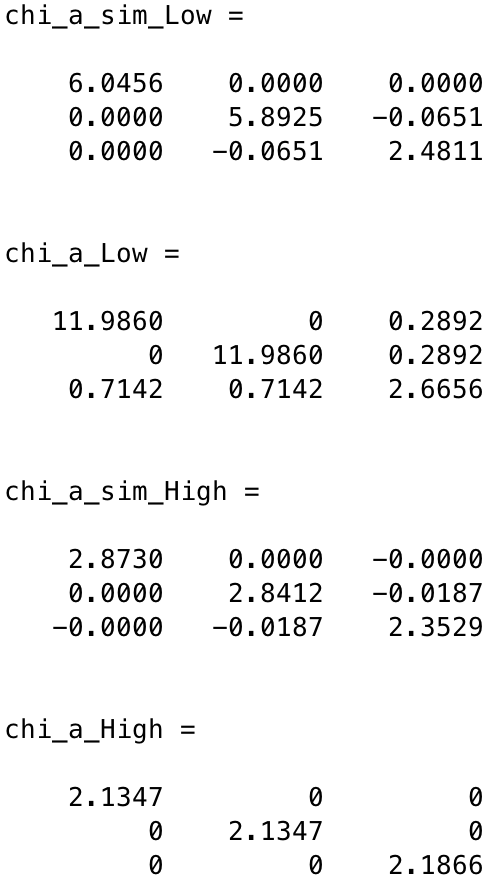
\includegraphics[width=0.25\textwidth]{Pictures/ExperimentalAssessk7chi.png}
	\caption{Comparison of simulation and experimental apparent susceptibilities for high and low fields for polycristalline nickel macrohelix (k = 7)}
	\label{fig:ExperimentalAssessk7chi}
\end{figure}

\begin{figure}[h]
	\centering
  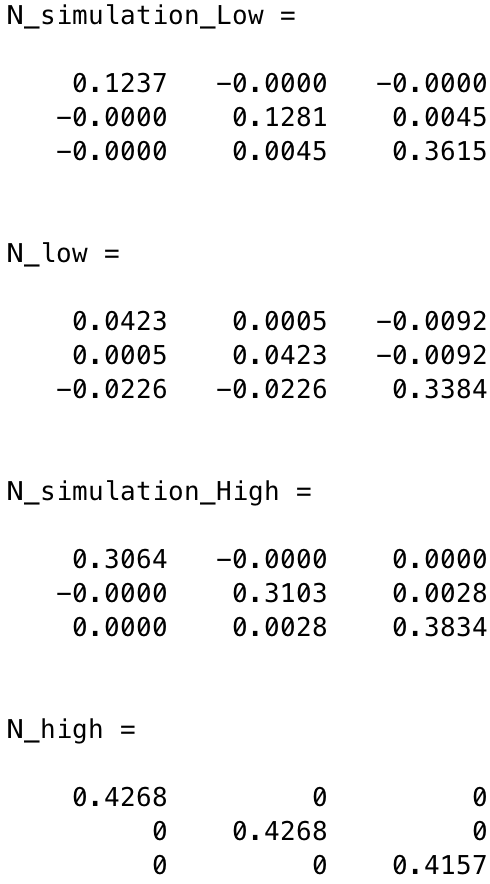
\includegraphics[width=0.25\textwidth]{Pictures/ExperimentalAssessk7N.png}
	\caption{Comparison of simulation and experimental demagnetization matrices for high and low fields for polycristalline nickel macrohelix (k = 7)}
	\label{fig:ExperimentalAssessk7N}
\end{figure}

\begin{figure}[h]
	\centering
  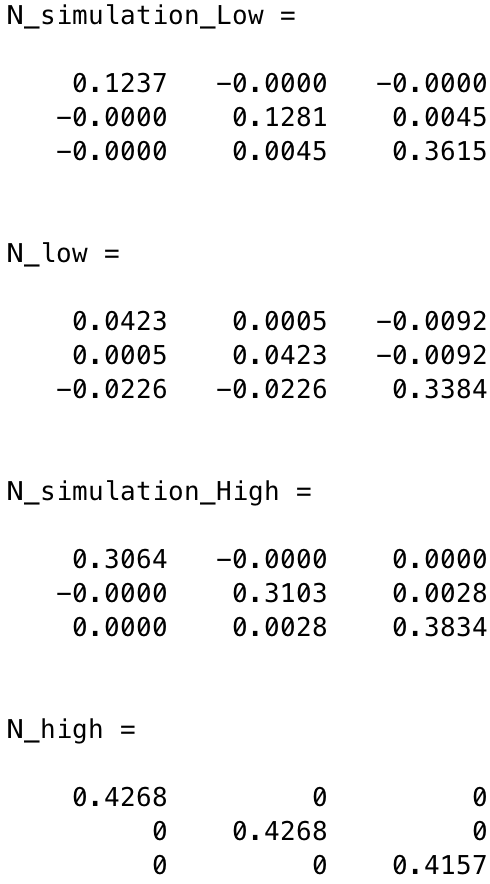
\includegraphics[width=0.25\textwidth]{Pictures/ExperimentalAssessk7N.png}
	\caption{Comparison of simulation and experimental demagnetization matrices for high and low fields for polycristalline nickel macrohelix (k = 7)}
	\label{fig:ExperimentalAssessk7N}
\end{figure}

\clearpage
\section{Setting up the simulation environment}

In this Section the three cases of simulations are going to be explained. The first two will be the means to the calculation of magnetic properties of a saturated magnetic shape. One setting up a fixed constant magnetization on the body, achieving this way an ideal saturation and skipping the step of actually magnetizing a shape and the second actually giving the body non-linear magnetic properties and subjecting it to very high fields. The third setup will be the simulation of low field magnetization, were we will give the body a linear magnetic property and then subject it to a field of some arbitrary magnitude. We will start by setting up the system for the shape and any magnetic calculations and we will go into the special details of every case separately.\\

\subsection{Adding the Physics}

We will start first by opening COMSOL and using the Model Wizard by clicking on ''New''. This part will help us set up the basics of the physics that are going to be used in COMSOL.\\

\begin{figure}[H]
	\centering
  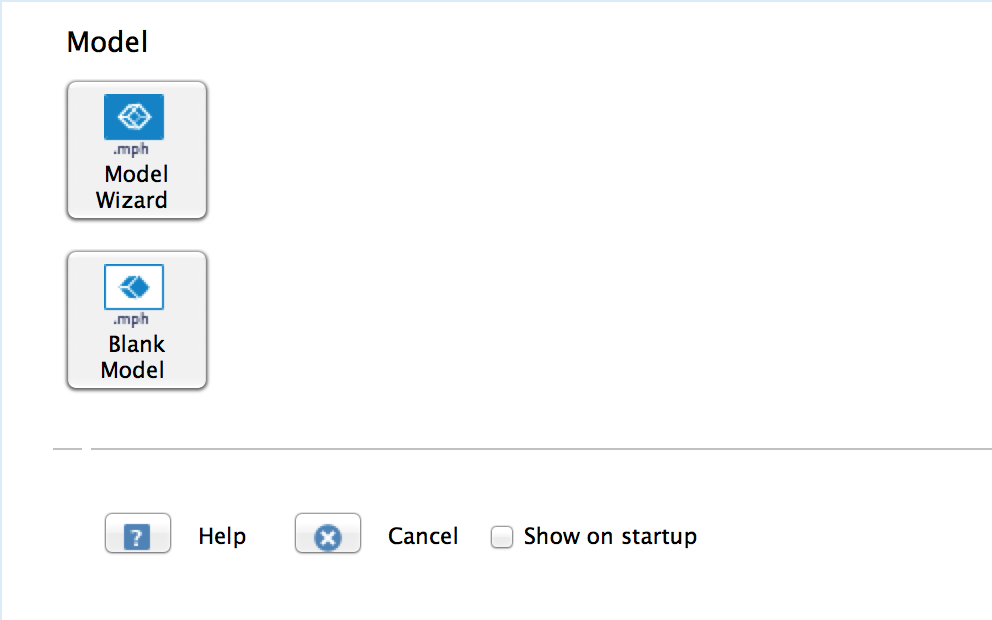
\includegraphics[width=0.6\textwidth]{Pictures/Screenshots/Sim1.png}
\end{figure}

After that, chose ''3D'' since we're going to be using a 3D model and simulation.\\

\begin{figure}[H]
	\centering
  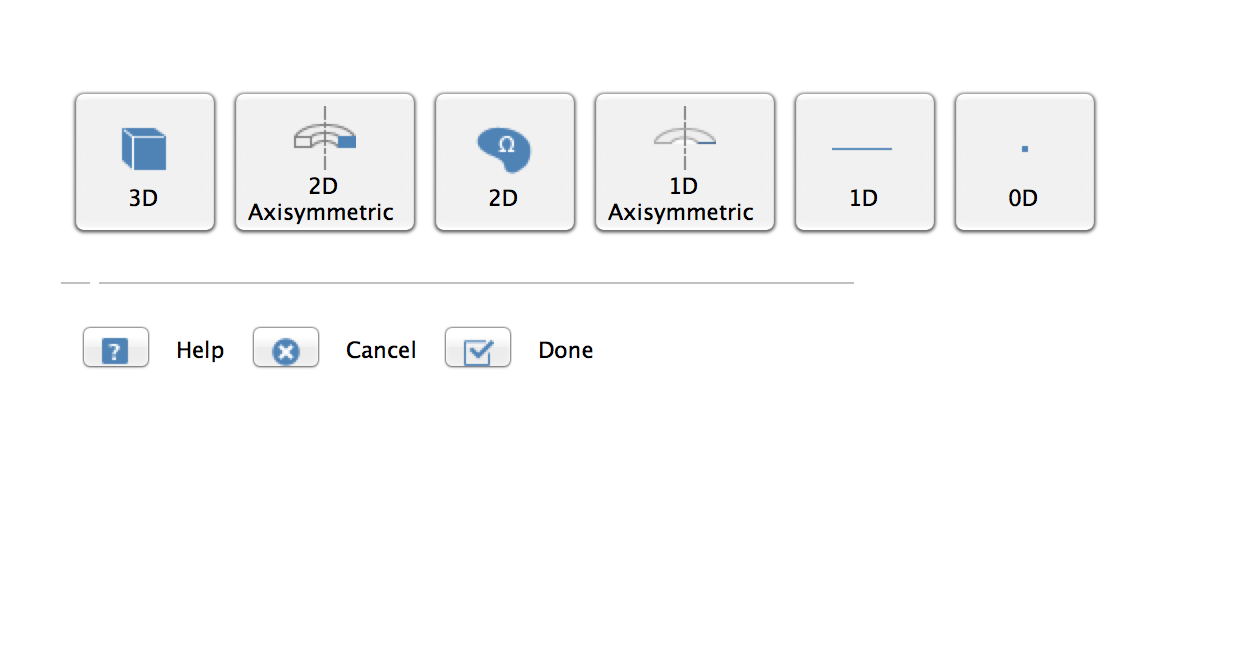
\includegraphics[width=0.6\textwidth]{Pictures/Screenshots/Sim2.png}
\end{figure}

The physics environment that is going to be used here is ''Magnetic fields, no currents (mfnc)''.\\

\begin{figure}[H]
	\centering
  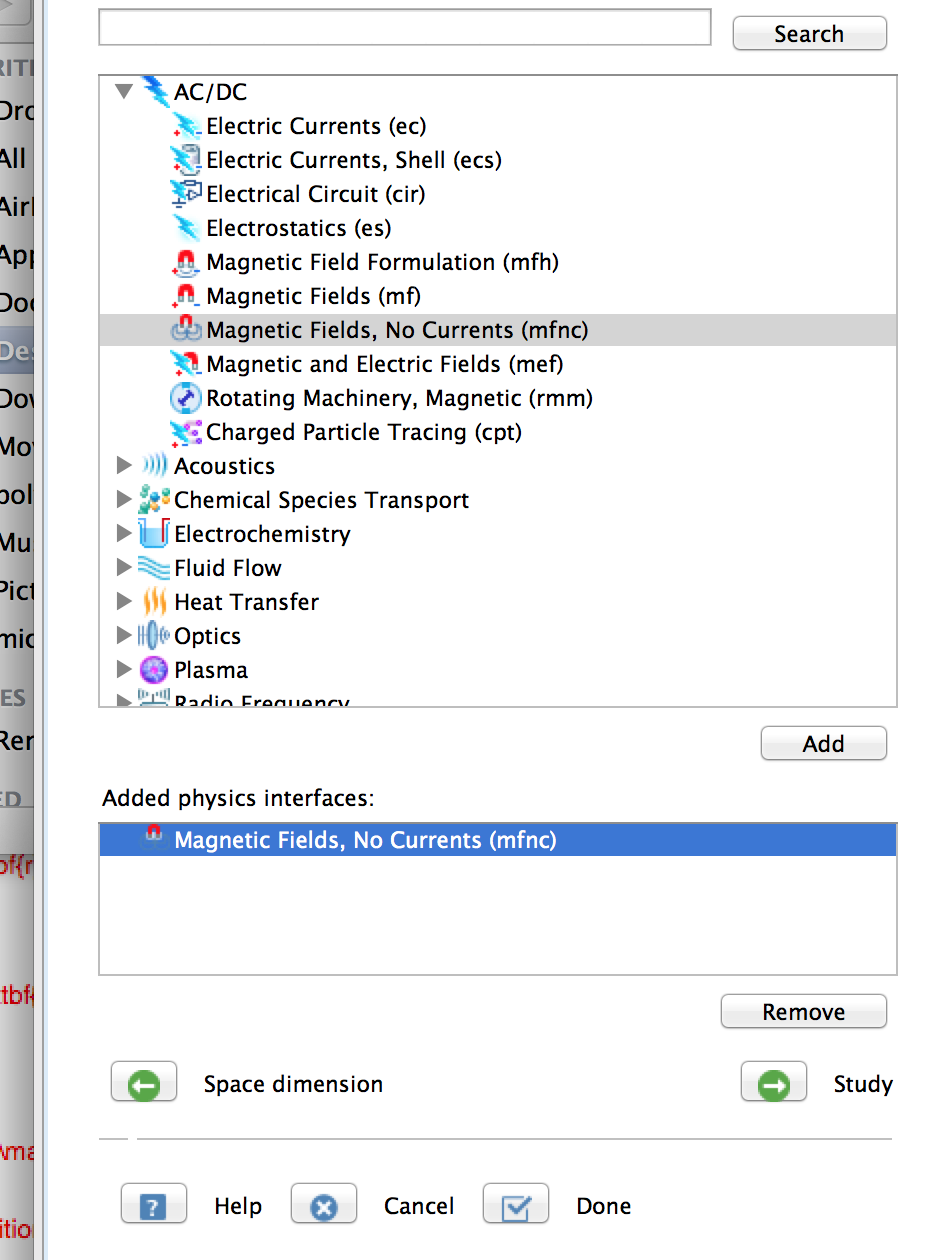
\includegraphics[width=0.4\textwidth]{Pictures/Screenshots/Sim3.png}
\end{figure}

Having this done, we continue by clicking on the ''Study'' button.\\

\begin{figure}[H]
	\centering
  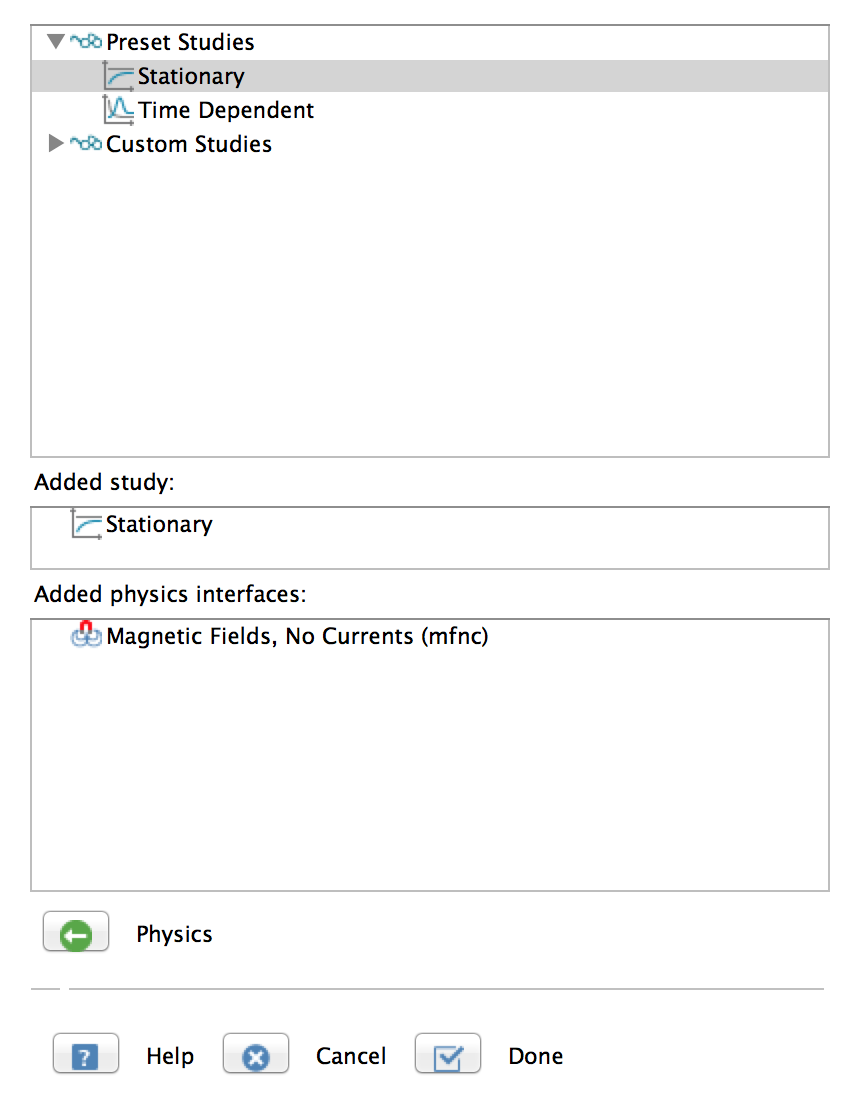
\includegraphics[width=0.3\textwidth]{Pictures/Screenshots/Sim25.png}
\end{figure}

Here we chose the ''Sationary'' preset study and then we finish the wizard by clickin in  ''Done''.

\begin{figure}[H]
	\centering
  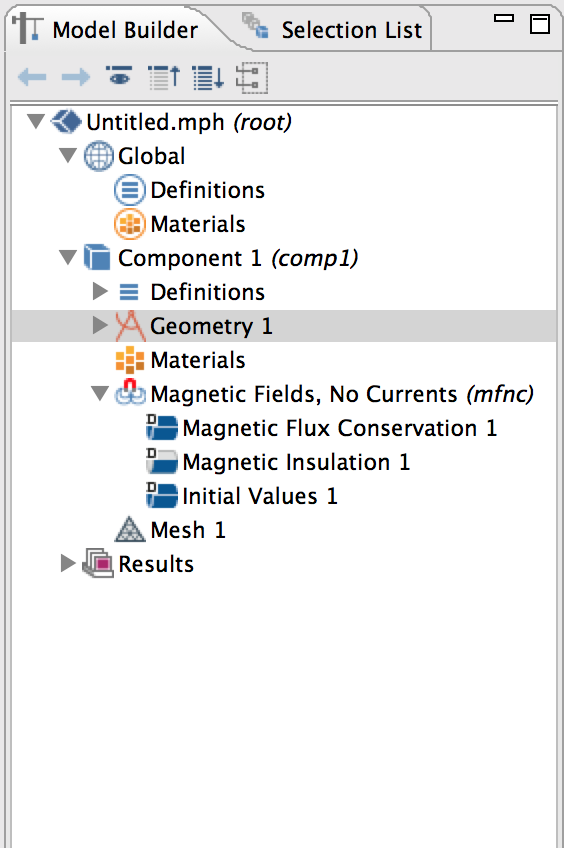
\includegraphics[width=0.4\textwidth]{Pictures/Screenshots/Sim4.png}
\end{figure}


\subsection{Adding the Geometry}

Adding the geomtry in COMSOL is a simple task that, as long as we're dealing with easy shapes or logical combinations (addition, substraction, etc.) of easy shapes, we can use the built-in functionalities of COMSOL. In this case we're going to show how to add a rectangular shape.\\

The first step is to go to the menu of Geometry by right-clicking on ''Geometry'' and selecting the desired Geometry, e.g. a helix or a block.\\

\begin{figure}[H]
	\centering
  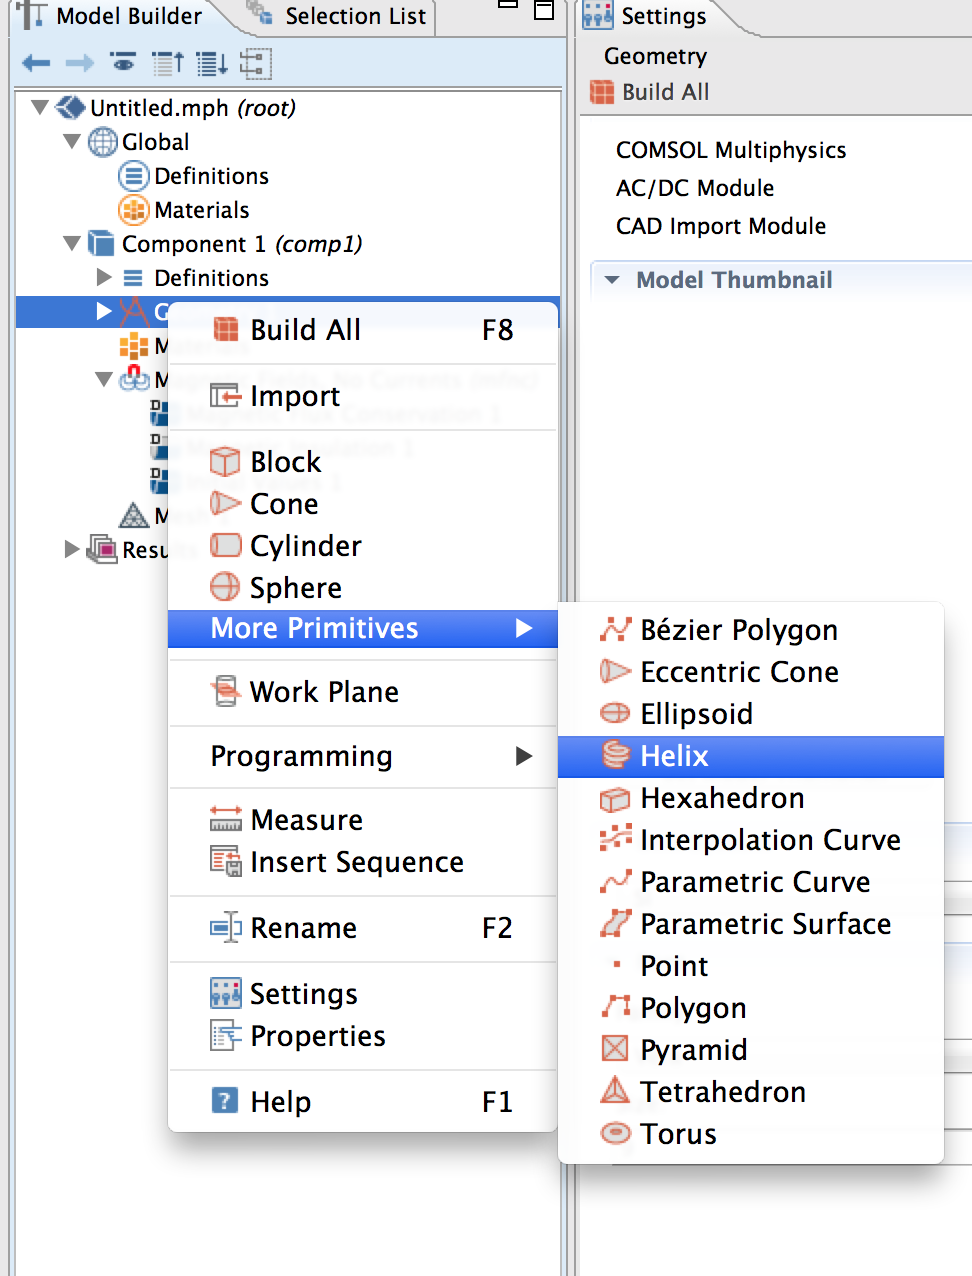
\includegraphics[width=0.4\textwidth]{Pictures/Screenshots/Sim5.png}
\end{figure}

This done, the geometrical properties of the desired shape have to be edited and finally the button ''Build selected'' or ''Build all objects'' has to be clicked.\\

\begin{figure}[H]
	\centering
  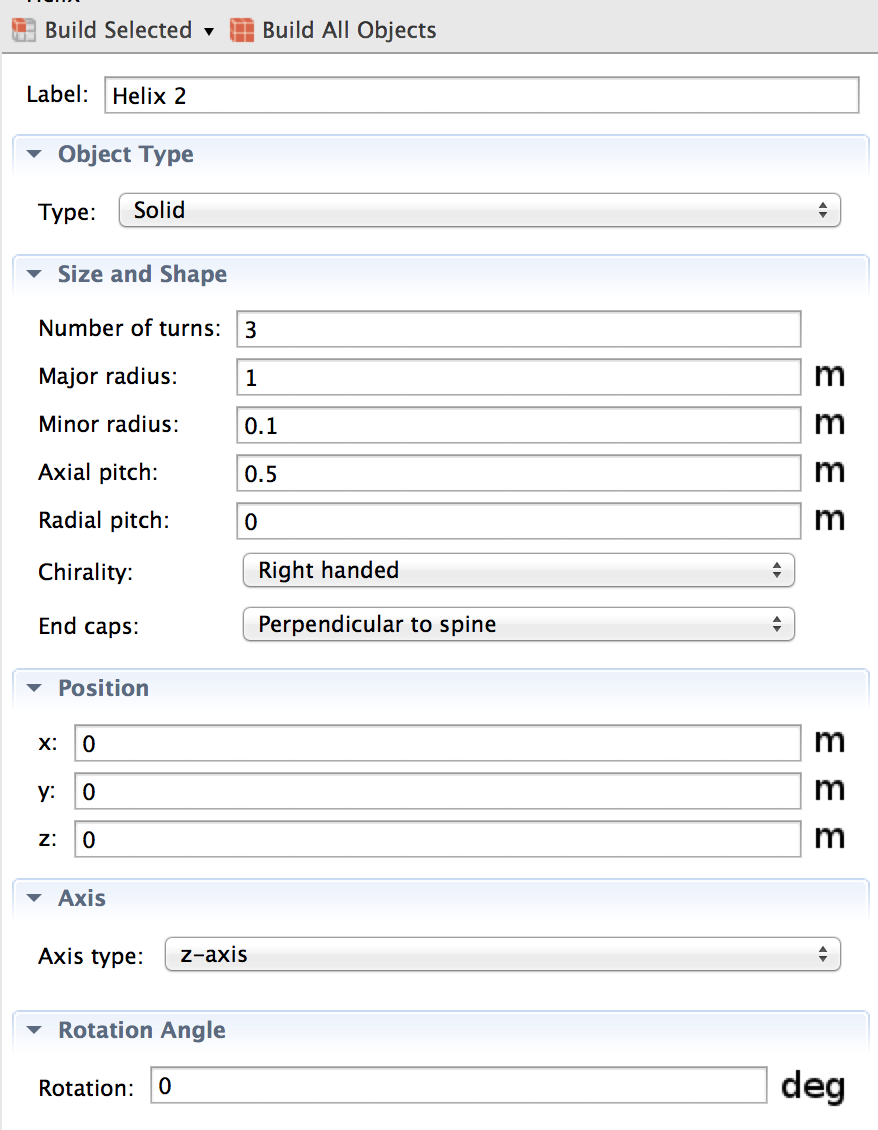
\includegraphics[width=0.4\textwidth]{Pictures/Screenshots/Sim6.png}
\end{figure}

In order to our FEM simulations to be run successfully, one has to define a system boundary. This can be done by creating a shape, bigger than the objects to be analysed to sorround the geometries and define the limits. In this case we used a sphere with its radius being five times the longest axial dimension of the helix. \\

\begin{figure}[H]
	\centering
  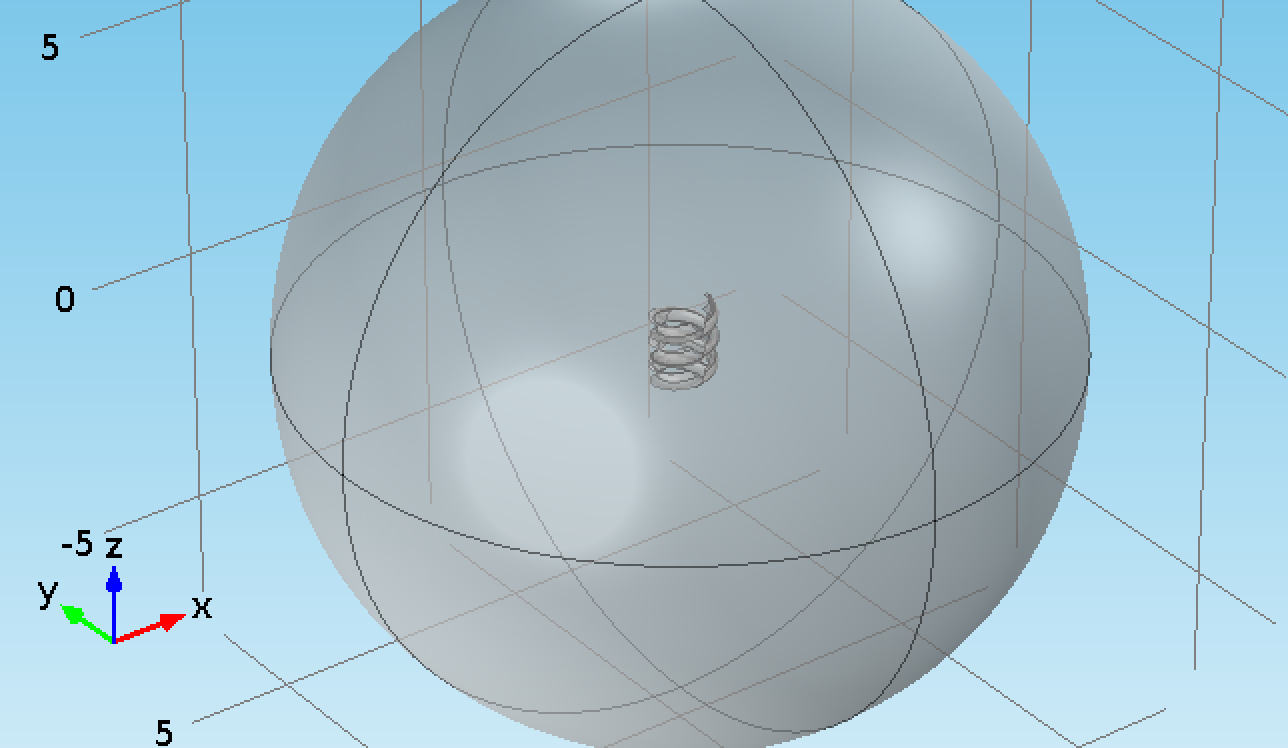
\includegraphics[width=0.4\textwidth]{Pictures/Screenshots/Sim8.png}
\end{figure}

\subsection{Adding a material}

To add a material, one has to click on the ''Material'' node and select ''Add material''.\\
 \begin{figure}[H]
\centering
 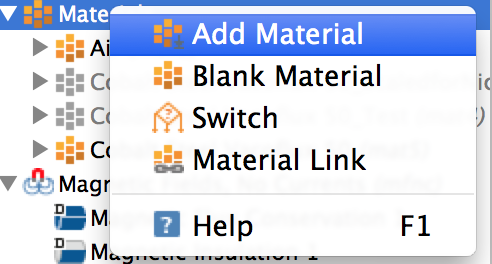
\includegraphics[width=0.4\textwidth]{Pictures/Screenshots/Sim14.png}
\end{figure}

Then out of the material library (using the search bar) one selects the desired material. Since we're going to assume the environment is non-magnetizable we will chose ''Air'' and then assign it with the selection tool to the environment shape.\\

 \begin{figure}[H]
\centering
 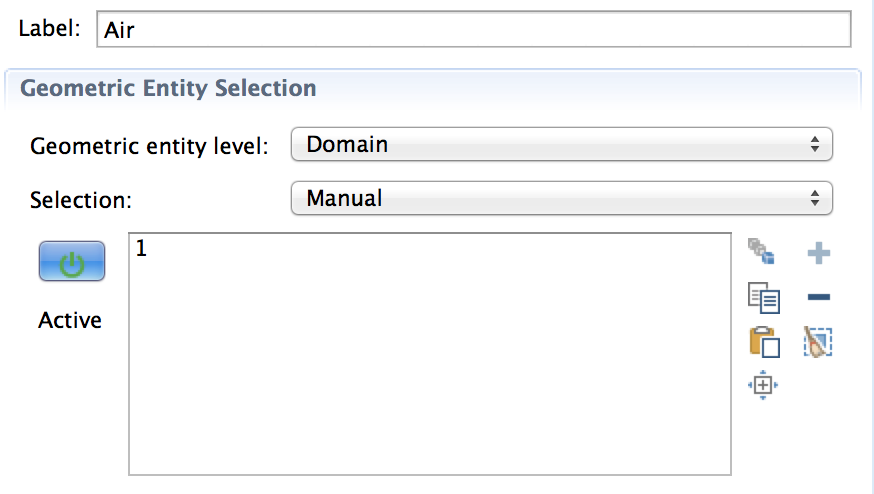
\includegraphics[width=0.4\textwidth]{Pictures/Screenshots/Sim15.png}
\end{figure}

\subsection{Magnetization Environments}

In this we're going to show the set-up of the different environments used in this thesis. The first one being the constant magnetization to simulate a perfect saturated material, the second one the actual saturation of a non-linear magnetic shape through high fields and the last one the linear magnetization of the shape to simulate the low-field case.\\

Since this type of magnetization problems are solved through the scalar magnetic potential, it is convenient to define a zero-level for it to help the solvers work more efficiently (sparing, thus, the solver the decision of the zero placement in the 3D space). To do this we do a right-click on the node ''Magnetic Fields, No Currents (mfnc)'' and we select ''Zero Magnetic Scalar Potential''.\\

\begin{figure}[H]
	\centering
  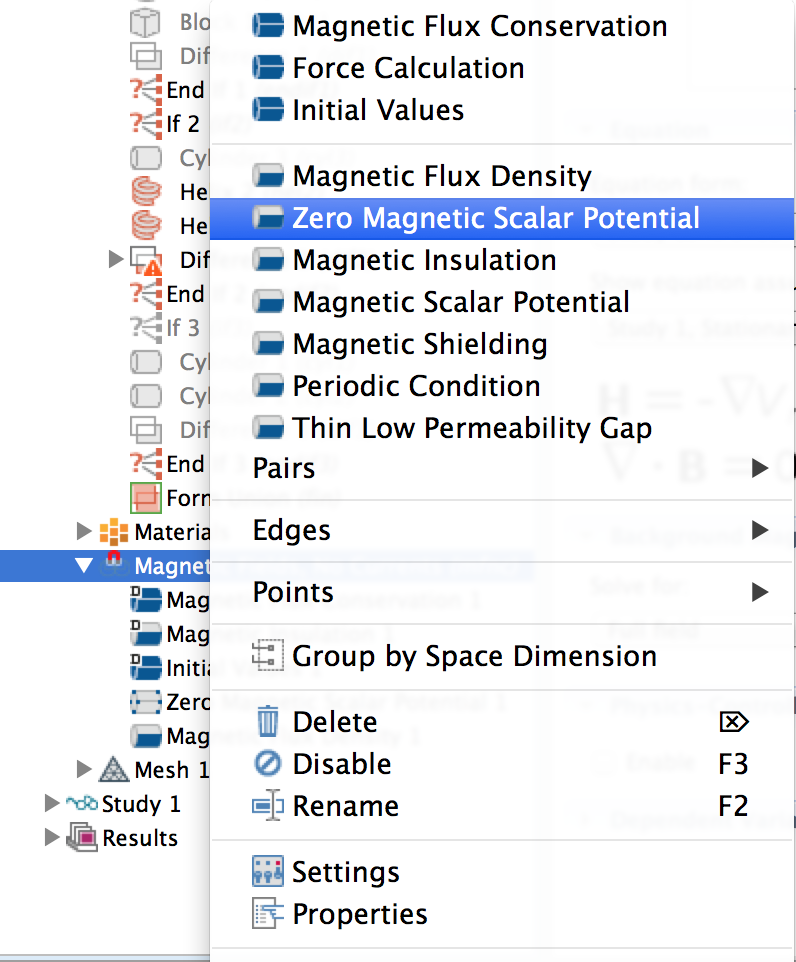
\includegraphics[width=0.4\textwidth]{Pictures/Screenshots/Sim7.png}
\end{figure}

Once the object is created, using the selection tool, one can select any arbitrary point in the geometries created before.

\begin{figure}[H]
	\centering
  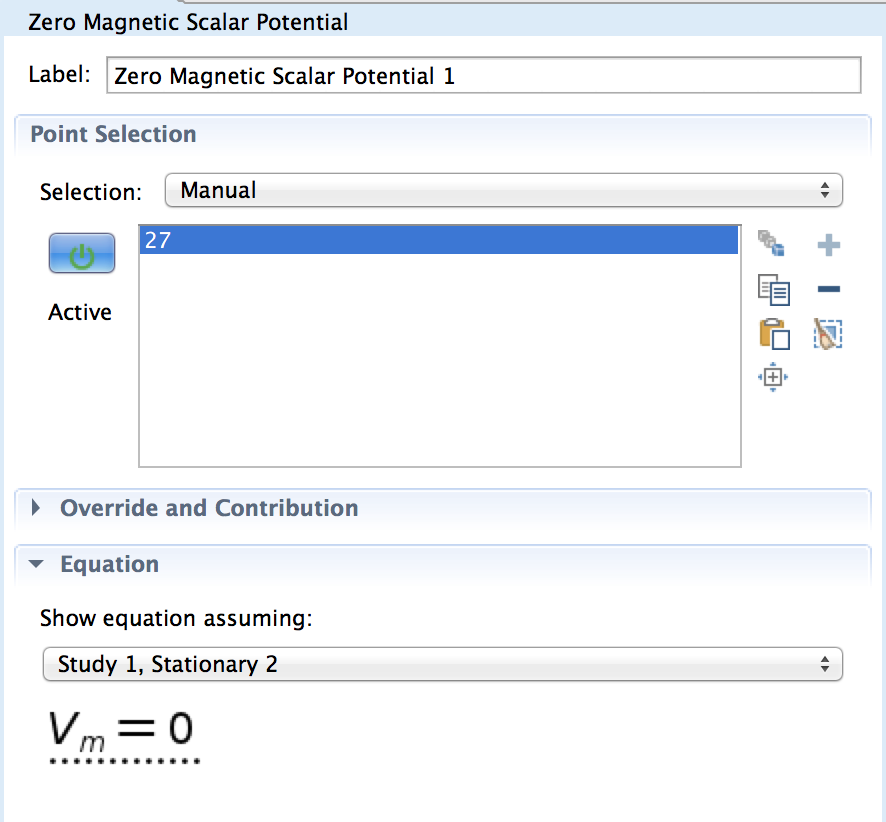
\includegraphics[width=0.4\textwidth]{Pictures/Screenshots/Sim9.png}
\end{figure}

 

\subsubsection{Linear Magnetization}

This will come first, since it's the easiest of the cases to set up. The only thing we have to do here is make sure that the relative permeability of the object is correct. By putting it in the correct field within the material selected for the shape\\
 
\begin{figure}[H]
	\centering
  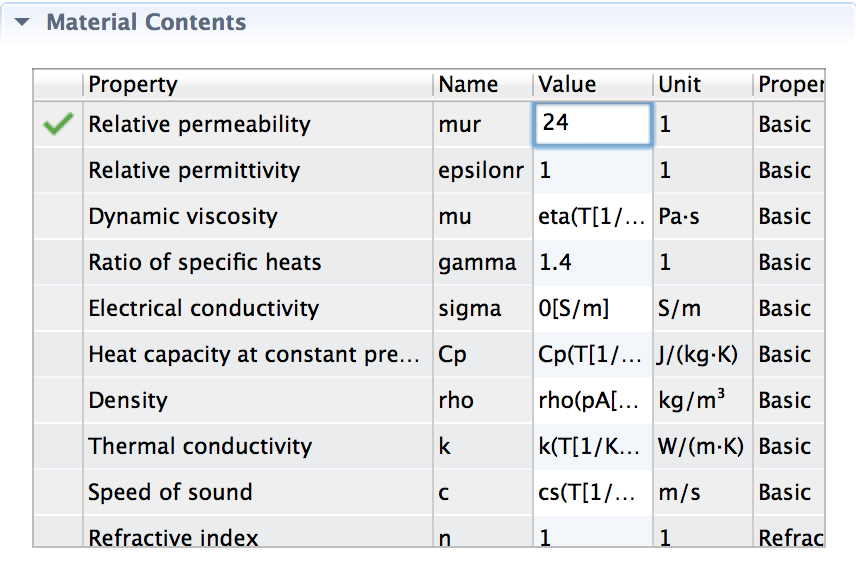
\includegraphics[width=0.4\textwidth]{Pictures/Screenshots/Sim13.png}
\end{figure}

Having done this, one has to make sure, that the existing object ''Magnetic Flux Conservation'' has in the selection editor both the environment shape and the shape to magnetize inside.\\

After that we have to set-up the external applied field. To do this we create a new magnetic object called ''Magnetic Flux Density''.\\

\begin{figure}[H]
	\centering
  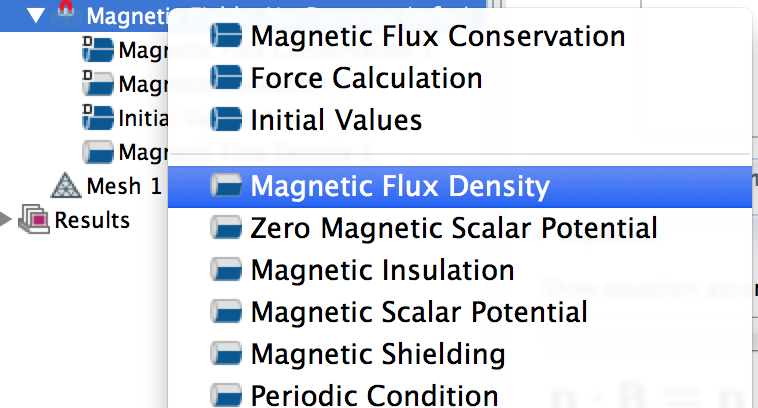
\includegraphics[width=0.4\textwidth]{Pictures/Screenshots/Sim17.png}
\end{figure}

Once created we make sure the environment shape is selected in the selection editor and then we change the picklist value ''Type'' to ''Magnetic Flux Density''. This being done, one can now chose the magnitude and direction of the applied external field under the title ''Magnetic Flux Density''.

\begin{figure}[H]
	\centering
  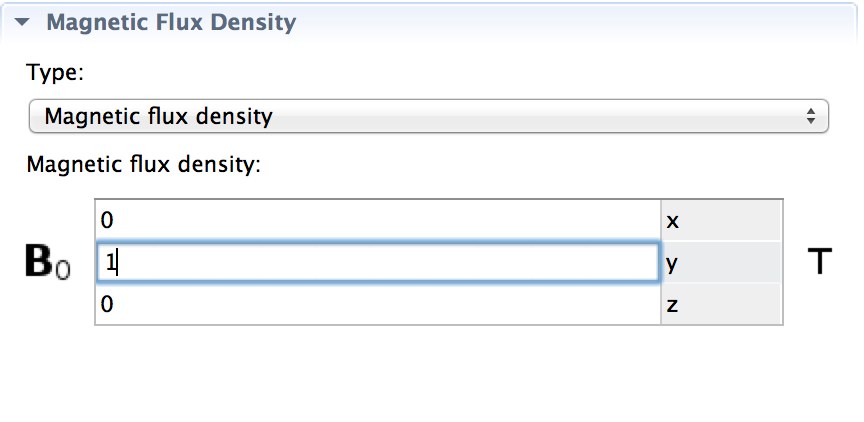
\includegraphics[width=0.4\textwidth]{Pictures/Screenshots/Sim18.png}
\end{figure}



\subsubsection{Constant Magnetization}

In this part we create a new magnetic object called ''Magnetic Flux Conservation''.\\

\begin{figure}[H]
	\centering
  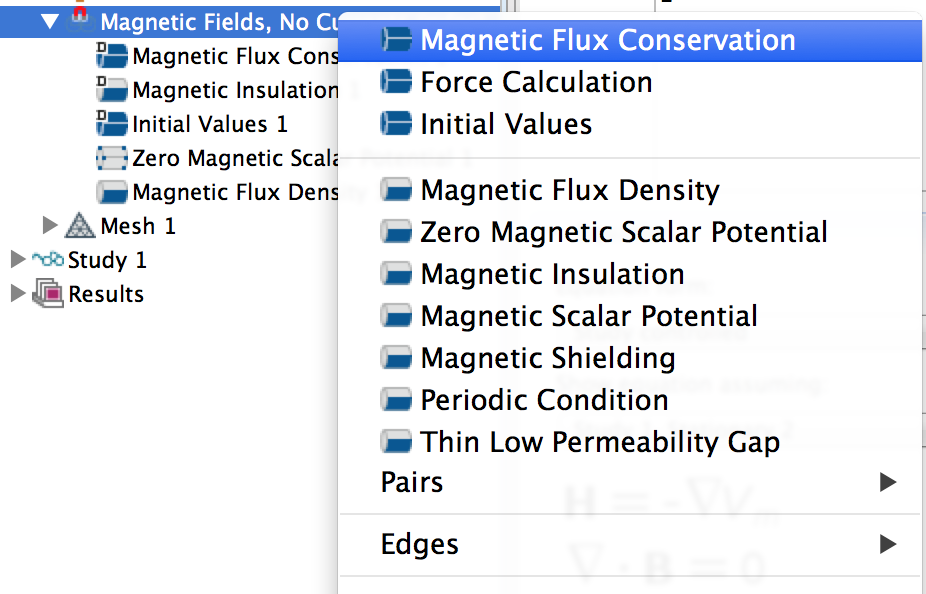
\includegraphics[width=0.4\textwidth]{Pictures/Screenshots/Sim10.png}
\end{figure}
 
In the properties of this object we make sure only the shape to be magnetized is selected (using the selection editor on top) and then we change the value of ''Constitutive Relation'' by selecting the picklist value ''Magnetization''. In the fields for the remanent magnetization we select a magnetization value for each direction to get our magnetized shape. \\

\begin{figure}[H]
	\centering
  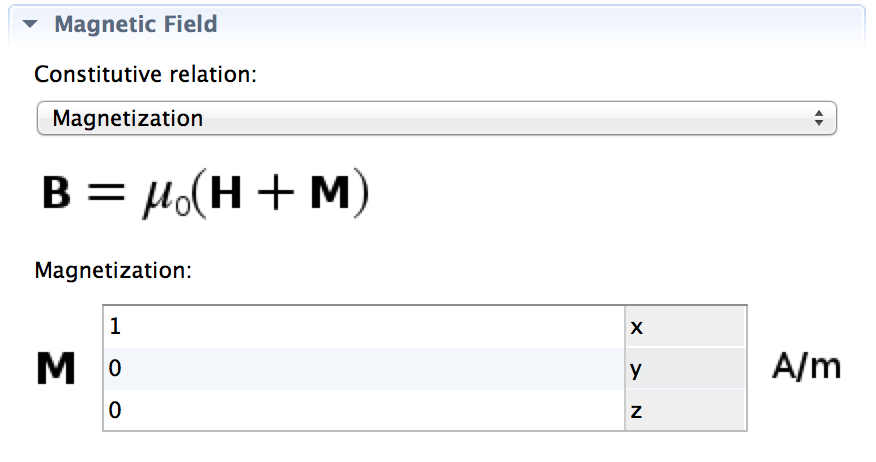
\includegraphics[width=0.4\textwidth]{Pictures/Screenshots/Sim11.png}
\end{figure}
 
 In this part there is no need for chosing any materials for the shape as well as an external applied field since we're dealing with the situation as if the magnetization (saturation) would already have happened.
 
\subsubsection{Saturation}

Starting from the same point we started in the section of Constant Magnetization, we have to create again the magnetic object 'Magnetic Flux Conservation''. We make sure, first, from the selection editor, that the right shape is chosen, namely the one that is going to get magnetized. This time we change the value of ''Constitutive Relation'' by selecting the picklist value ''BH Curve''. A new picklist appears with the name ''Magnetic flux density norm'' and its value has to be `'From Material''

\begin{figure}[H]
	\centering
  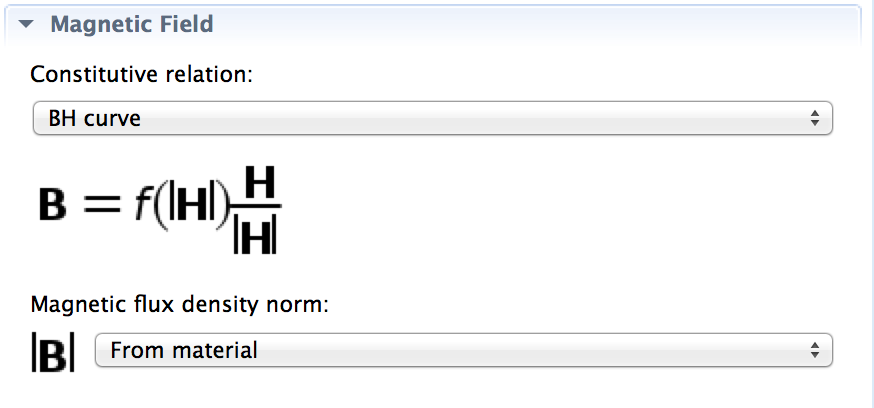
\includegraphics[width=0.4\textwidth]{Pictures/Screenshots/Sim12.png}
\end{figure}

No we have to make sure that the material has the right magnetization curve (BH Curve) so that the simulation is correct. For that we go to the material node and create a new material. In the material library we go to the Non-linear magnetic section and select any material of our choice.\\

 \begin{figure}[H]
	\centering
  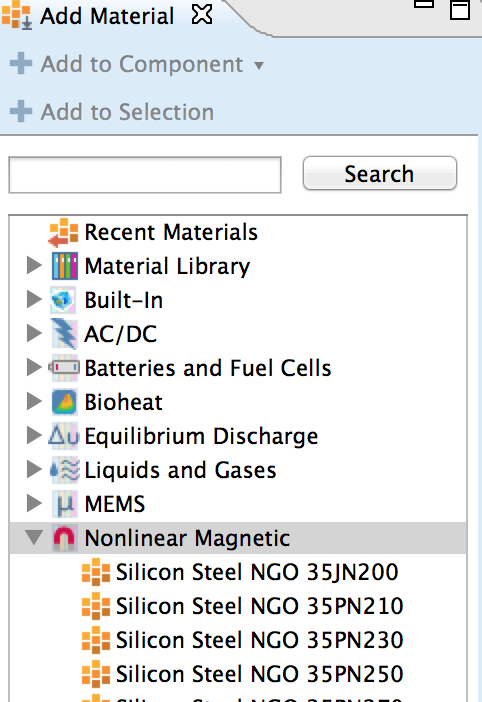
\includegraphics[width=0.4\textwidth]{Pictures/Screenshots/Sim16.png}
\end{figure} 

The reason for this freedom of choice is only that we want to saturate the material. The curve itself, doesn't really interest us, but we rather just need the saturation behaviour to do our calculations, since we want to calculate the demagnetization factor (which is a shape factor).\\

What is now left is to create the applied field the way it was created in the section for Linear Magnetization this time making sure the magnitude of the field is big enough, e.g. 5000 Tesla.

\subsection{Meshing}

To create a Mesh node one has to do a right click on the Component node and click on ''Add Mesh''.

 \begin{figure}[H]
	\centering
  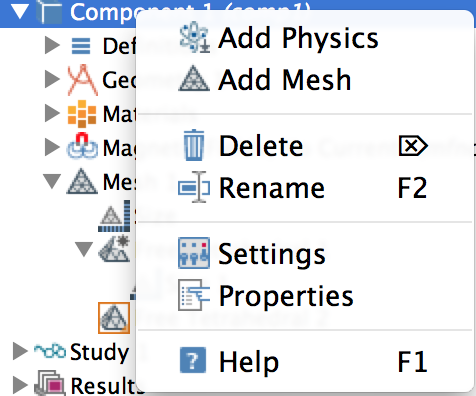
\includegraphics[width=0.4\textwidth]{Pictures/Screenshots/Sim19.png}
\end{figure} 

 The meshing properties of the environment and the meshing properties of the shape itself. To set this up one has to create the following objects in the Mesh node (by doing a right click on it): One size object and two ''Free Tetrahedral'' objects at the same level of the hierarchy and one ''Size'' object inside the second ''Free Tetrahedral'' object

 \begin{figure}[H]
	\centering
  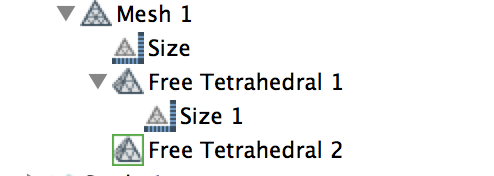
\includegraphics[width=0.4\textwidth]{Pictures/Screenshots/Sim20.png}
\end{figure} 

For the meshing process there is two decisions that have to be made. The refinement of the mesh for the environment and the refinment of the mesh for the shape. For it to have the proper assignments the properties have to be set as shown in the illustrations. \\

For the first ''Size object'':\\
 \begin{figure}[H]
	\centering
  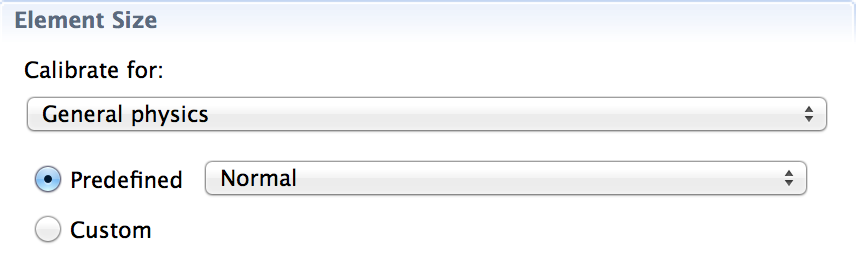
\includegraphics[width=0.4\textwidth]{Pictures/Screenshots/Sim21.png}
\end{figure} 


For the first ''Free Tetrahedral'' object:\\
 \begin{figure}[H]
	\centering
  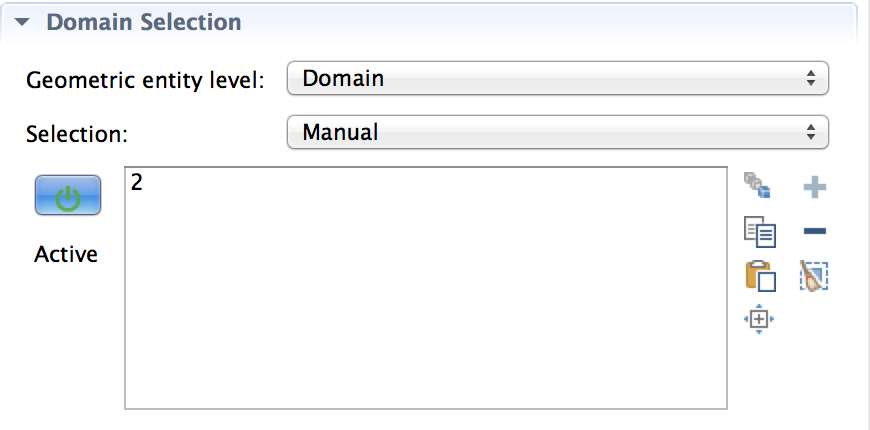
\includegraphics[width=0.4\textwidth]{Pictures/Screenshots/Sim22.png}
\end{figure} 


For the second ''Size'' object\\
\begin{figure}[H]
	\centering
  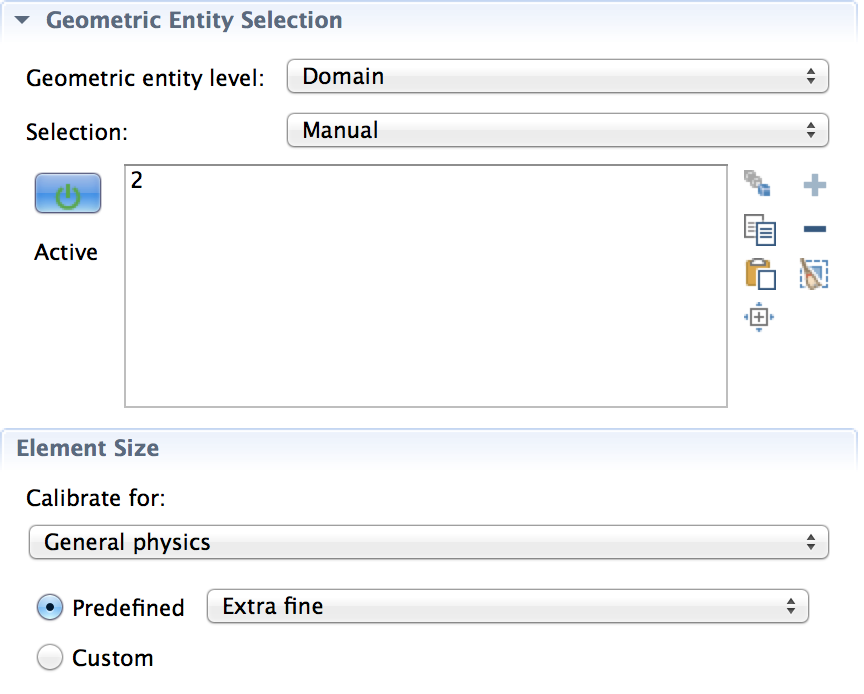
\includegraphics[width=0.4\textwidth]{Pictures/Screenshots/Sim23.png}
\end{figure} 

For the second ''Free Tetrahedral'' object:\\
\begin{figure}[H]
	\centering
  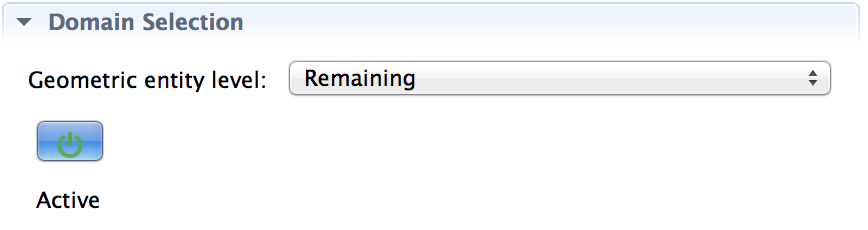
\includegraphics[width=0.4\textwidth]{Pictures/Screenshots/Sim24.png}
\end{figure} 

\subsection{Calculating}

To activate the simulation one will have to do a right click on the ''Study'' node and click on ''Compute''.

\begin{figure}[H]
	\centering
  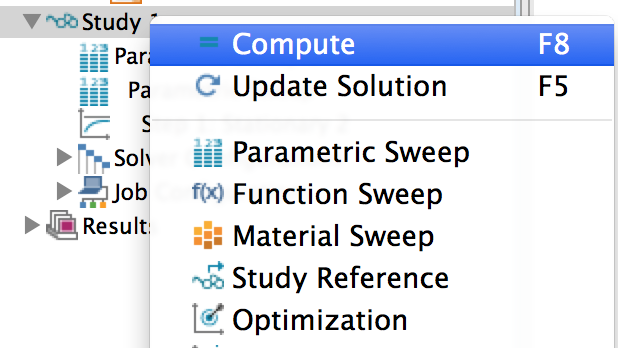
\includegraphics[width=0.4\textwidth]{Pictures/Screenshots/Sim26.png}
\end{figure} 


\subsubsection{Parametric Sweeps}

Since for our calculations we will need to do always a simulation for three linearly independent directions, we will need the functionality of Parametric Sweeps to work efficiently. This allows us to calculate the three directions within the same process and then export them to Matlab as one single process (instead of three).\\

The way to set it up is to create a ''Parametric Sweep'' object from within the ''Study Node''.\\
\begin{figure}[H]
	\centering
  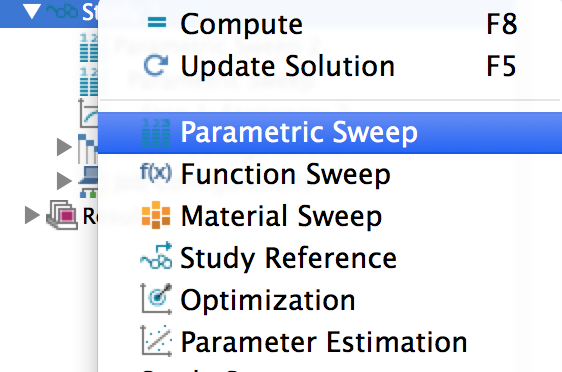
\includegraphics[width=0.4\textwidth]{Pictures/Screenshots/Sim27.png}
\end{figure} 

The next step is to chose the variable or variables that have to change value in each of the different processes. In this case we chose the variables $B_x$, $B_y$ and $B_z$ defined in the global parameters and we assign the values they have to have in each of the processes in the following way:\\

\begin{figure}[H]
	\centering
  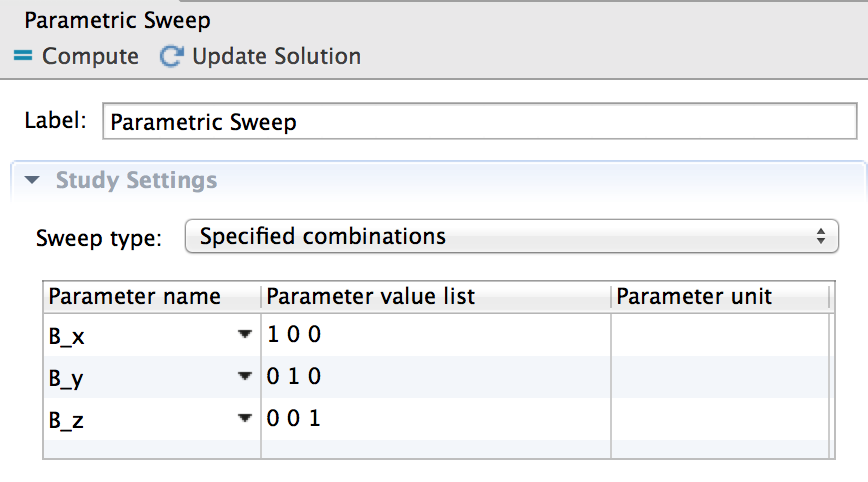
\includegraphics[width=0.4\textwidth]{Pictures/Screenshots/Sim28.png}
\end{figure} 

The variables are then put in the fields for the applied field within the ''Magnetic Flux Density'' object.\\
\begin{figure}[H]
	\centering
  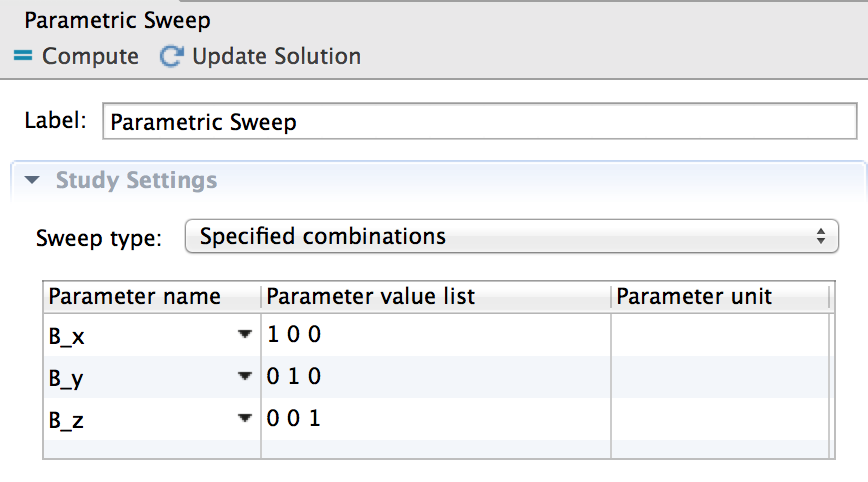
\includegraphics[width=0.4\textwidth]{Pictures/Screenshots/Sim28.png}
\end{figure} 

It is important to know that Parametric Sweeps are a very powerful tool that allows to nest various Parametric Sweeps within each other in case one wants to do, for example, this type of calculation for three different directions at the same time for various different shape parameters (like in the case of the helices). In this case the parameter to be changed from cycle to cycle has to be defined the way the variables were defined in the above case and one would nest one Parametric Sweep inside the other.

\subsection{Postprocessing in Matlab}

In this module we will show the most important functionalities to import solutions of magnetic simulations from COMSOL into Matlab, such that the rest of the calculations and plotting (postprocessing) can be done in Matlab.\\

The first step to do is to open the COMSOL Multiphysics Server before Matlab is opened.\\

\begin{figure}[H]
	\centering
  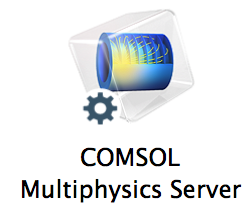
\includegraphics[width=0.2\textwidth]{Pictures/Screenshots/Sim30.png}
\end{figure} 

Doing this, the terminal will open and will confirm if the server could have been opened and in which port it is listening (usually port 2036):

\begin{figure}[H]
	\centering
  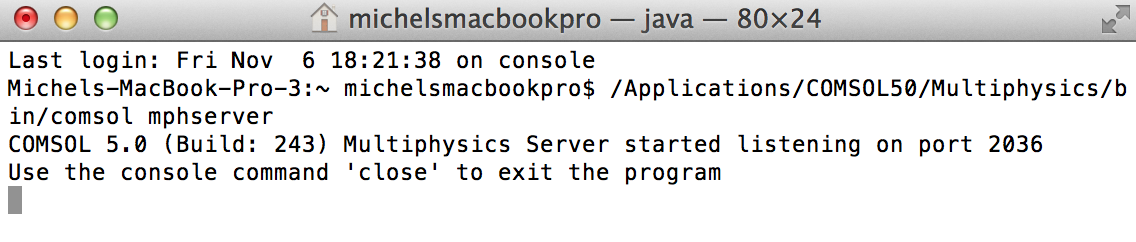
\includegraphics[width=0.8\textwidth]{Pictures/Screenshots/Sim31.png}
\end{figure} 

The first line that has to be input in Matlab (only one time) is \textit{mphstart(2036)} where the number inside has to be the same one given in the terminal console. This will initializate the connection between the COMSOL environment and Matlab.

\begin{figure}[H]
	\centering
  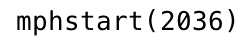
\includegraphics[width=0.2\textwidth]{Pictures/Screenshots/Sim32.png}
\end{figure} 

After this one has to load the already simulated model to Matlab. To have a view of the nodes inside the loaded model one can always use the \textit{mphnavigator} to see them whithin Matlab, so there is no necesity of opening the model in COMSOL.

\begin{figure}[H]
	\centering
  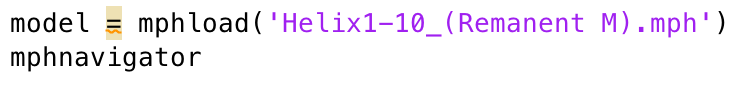
\includegraphics[width=0.7\textwidth]{Pictures/Screenshots/Sim33.png}
\end{figure} 

Once the model has been loaded, the solutions within the model can be downloaded. Since we're dealing with averaged values over the whole shape we use the function \textit{mphmean}. The first argument refers to the previously loaded model. The second argument is a list of the variables (including solution variables) to be extracted from the models. These are extracted to the function outputs at the beginning of the line. The third argument states we are dealing with a volume average over the selection 2, which is the magnetized shape (selection 1 would be the environment sphere) the following two arguments state the selection of the dataset used (coming from the solution). To see the data set that is being used, one has to look it up in the solution node of the \textit{mphnavigator}. The last two inputs state the index of the solution within the outermost parameter sweep (in case there is one). In the case of having two Parameter Sweeps, this would refer to the outmost and the rest of the exported variables would have three values according to each one of the solutions (for each direction of the applied field).\\

\begin{figure}[H]
	\centering
  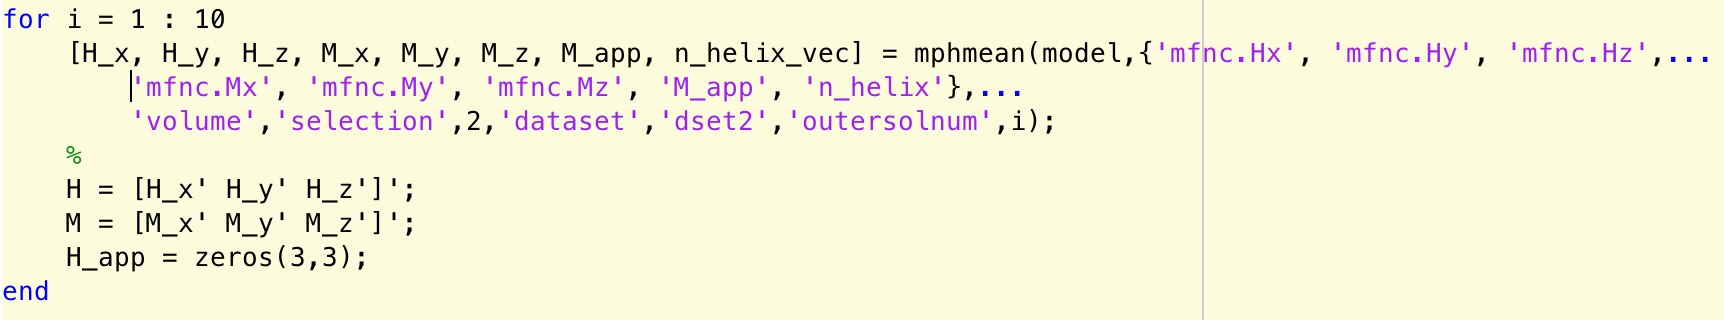
\includegraphics[width=\textwidth]{Pictures/Screenshots/Sim34.png}
\end{figure} 

Once this is done the matrices of the applied field (in this case zero, since we're dealing with the method were the magnetization is set as constant), the magnetization and the total H-field can be constructed according to the way it was defined in this thesis and then further calculations can be done. 

\section{Running Matlab Scripts with BRUTUS}

Before one uses BRUTUS, one has to contact the administrator to be sure to have an account on it. It is also recommended to have a FTP client (e.g. Filezilla) to manage the files in BUTUS. Provided this, one can continue with the specific steps.\\

Provided one is connected to the ETH network, either through wireless or through VPN, one can connect to the cluster with the next line:\\

\textit{ssh [username]@brutus@ethz.ch}\\

After having entered the password, te connection will have been set up properly

\begin{figure}[H]
	\centering
  \includegraphics[width=\textwidth]{Pictures/Screenshots/Sim35.png}
\end{figure} 

The next step is to load the Matlab module to be able to run Matlab scripts. For this one should use the line:\\

\textit{module load matlab}\\

Having this done. The important step now is to get the files to the server using a ftp manager. The direction is:\\

\textit{sftp://[username]@brutus.ethz.ch}\\

It is important to know the folder hierarchy within the sftp so that you know how to access it with unix commands through the command screen.

\begin{figure}[H]
	\centering
  \includegraphics[width=\textwidth]{Pictures/Screenshots/Sim36.png}
\end{figure} 

If, for example, I have my scripts under the folder called ''Calculations'' I type:\\

\textit{cd Calculations}\\

in the command line and then \textit{ls} to see the files within that folder. Once that one is in the desired folder one can send the job in the following way:\\

\textit{bsub -W "24:00" -R "rusage[mem=1500]" matlab -nodisplay -nojvm -singleCompThread -r simulation}\\

Where \textit{-W "24:00"} sets the time limit as 24 hours for the job, \textit{-R "rusage[mem=1500]"} sets the memory usage to 1.5 GB for the job, \textit{-nodisplay} supresses graphical objects, \textit{-nojvm} suppresses the java virtual machine (use this if you're not doing parallel jobs) \textit{-singleCompThread} is for non-parallel jobs and finally \textit{-r simulation} refers to the file \textit{simulation.m}.\\

Once this is done the job gets put in line and depending on how busy the cluster might be it can take up to a day until the job starts. Once the job ends, all output of the scripts can be found in the same file as the script. It is therefore very important to have file ouptputs from the script (e.g. saving to .mat files). If the job breaks because of compilation errors, one can find the log in the same file where the outputs of the Command Window of Matlab can be seen.



